% !TeX program = tectonic
\documentclass[%
  paper=a4,
  fontsize=11pt,
  BCOR=8mm,
  DIV=12,
  headings=normal,1
  parskip=half,
  numbers=noendperiod
]{scrreprt}

% Fonts & language: Tectonic uses (Xe)TeX engine; use fontspec + polyglossia
% Encoding (safe default)
\usepackage[T1]{fontenc}
\usepackage[utf8]{inputenc}

% Languages (replacement for polyglossia)
\usepackage[ngerman,british]{babel}

% TeX Gyre fonts (same fonts as before)
\usepackage{tgpagella}   % serif (main)
\usepackage{tgheros}     % sans-serif
\usepackage{tgcursor}    % monospace

% Make sans-serif the default sans font (optional but matches fontspec behaviour)
\renewcommand{\familydefault}{\rmdefault}
% Encoding & micro-typography
\usepackage{microtype}

% Graphics, tables, math (lightweight defaults)
\usepackage{graphicx}
\usepackage{booktabs}
\usepackage{siunitx}
\usepackage{amssymb}
\usepackage{amsmath}

\usepackage{pifont}
\sisetup{locale=US, detect-all}

% Bibliography with biblatex + biber
\usepackage[
  backend=biber,
  style=ieee
]{biblatex}
\addbibresource{bib/references.bib}

% Load hyperlink setup
\usepackage{xcolor}
\usepackage{hyperref}
\hypersetup{
    colorlinks=true,
    linkcolor=blue,
    citecolor=black,
    filecolor=magenta,      
    urlcolor=blue,
    pdftitle={Algorithmic Texture Synthesis: Procedural, Rule-Based and Optimization-Based Methods in Computer Graphics},
    pdfauthor={Eldar Omerovic},
    pdfsubject={Bachelor Thesis – Lucerne University of Applied Sciences and Arts, Department of Computer Science},
    pdfkeywords={algorithmic texture synthesis, procedural texturing, rule-based systems, optimization, parameter estimation, computer graphics, texture modeling},
    pdfpagemode=UseOutlines,
}
\urlstyle{same}

% Redefine the url command for the TOC to remove styling
\AtBeginDocument{
  \addtocontents{toc}{\protect\hypersetup{linkcolor=.,citecolor=black,urlcolor=.}}
}

% Load project preamble/macros
% Figure paths
\graphicspath{{figures/}}

% Klickbar: kompletter Eintrag (Text + Seitenzahl)
\hypersetup{linktoc=all}

% Hierarchie mit Einrückungen
\KOMAoptions{toc=graduated}

% Dichtes Punktmuster für die Leader
\makeatletter
\renewcommand*\TOCLineLeaderFill{\leaders\hbox to .6em{\hss.\hss}\hfill}
\makeatother

% No indentation, space between paragraphs
\setlength{\parindent}{0pt}
\setlength{\parskip}{\baselineskip}

\usepackage{csquotes}

\usepackage{listings}
\usepackage{xcolor}

\usepackage{upquote}
\usepackage{microtype}

\usepackage{float}

% --------------------
% Fonts & Typografie
% --------------------
\usepackage[T1]{fontenc}
\usepackage{lmodern}
\usepackage{microtype}

\usepackage{setspace}
\setstretch{1}

% Table that wraps over pages
\usepackage{longtable}
\usepackage{paracol}
\usepackage{array}

% listings

\usepackage{tocloft}
\usepackage[acronym]{glossaries}
\makeglossaries
\renewcommand*{\glstextformat}[1]{#1}

\renewcommand{\listfigurename}{List of Figures}
\renewcommand{\listtablename}{List of Tables}
\renewcommand{\lstlistlistingname}{List of Sources}


\makeatletter
\newcommand{\onlylof}{\@starttoc{lof}}
\newcommand{\onlylot}{\@starttoc{lot}}
\newcommand{\onlylol}{\@starttoc{lol}}
\makeatother

\usepackage{seqsplit}

\newcolumntype{P}[1]{>{\raggedright\arraybackslash\sloppy}p{#1}}
\newcommand{\cw}[1]{\seqsplit{#1}} % code-wrap helper

\usepackage{tabularx}
\usepackage{pdfpages}



\newacronym{uv}{UV}{Texture Coordinates}
\newacronym{3d}{3D}{Three-Dimensional}
\newacronym{gpu}{GPU}{Graphics Processing Unit}
\newacronym{fbm}{fBm}{fractal Brownian motion}
\newacronym{ai}{AI}{Artificial Intelligence}
\newacronym{nf}{NF}{Non-Functional}
\newacronym{id}{ID}{Identifier}
\newacronym{api}{API}{Application Programming Interface(s)}
\newacronym{ui}{UI}{User Interface}
\newacronym{wgsl}{WGSL}{WebGPU Shading Language}
\newacronym{cpu}{CPU}{Central Processing Unit}
\newacronym{css}{CSS}{Cascading Style Sheets}
\newacronym{c4}{C4}{Context, Containers, Components, and Code model}
\newacronym{c2}{C2}{C4 model level 2 / Container level}
\newacronym{c1}{C1}{C4 model level 1 / Context level}
\newacronym{c3}{C3}{C4 model level 3 / Component level}
\newacronym{csv}{CSV}{Comma-Separated Values}
\newacronym{fps}{FPS}{Frames Per Second}
\newacronym{ram}{RAM}{Random Access Memory}
\newacronym{pdca}{PDCA}{Plan-Do-Check-Act}
\newacronym{ddr5}{DDR5}{Double Data Rate 5}
\newacronym{pdf}{PDF}{Portable Document Format}
\lstdefinestyle{defaultcode}{
  basicstyle=\ttfamily\small,
  backgroundcolor=\color{gray!5},
  frame=single,
  rulecolor=\color{gray!40},
  breaklines=true,
  breakatwhitespace=true,
  tabsize=2,
  numbers=left,
  numberstyle=\tiny\color{gray!70},
  numbersep=8pt,
  captionpos=b,
  showstringspaces=false,
  columns=fullflexible,
  keepspaces=true,
  upquote=true
}

\lstset{style=defaultcode}
\newcommand{\img}[3][]{%
  \centering
  \includegraphics[#1]{#2}
  \caption{#3}
}

% Title meta
\title{Algorithmic Texture Synthesis}
\subtitle{Procedural, Rule-Based and Optimization-Based Methods in Computer Graphics}
\author{Eldar Omerovic}
\date{\today}

\begin{document}

\thispagestyle{empty}
\begin{center}
    
    \begin{flushleft}
        
\includegraphics[width=4cm]{titlepage/HSLU_Logo.png}
    \end{flushleft}

    \vspace{5cm}

    \noindent\makebox[\linewidth]{\rule{\textwidth}{1pt}} 
    
    \begin{center}
        \Large \textbf{Algorithmic Texture Synthesis}\\[5pt]
        \large Procedural, Rule-Based and Optimization-Based Methods in Computer Graphics\\
    \end{center}
    
    \noindent\makebox[\linewidth]{\rule{\textwidth}{1pt}} 
    
    \vspace{1cm}
    
    \begin{center}
    
    \textbf{Author}\\
    \textit{Eldar Omerovic}
    
    \vspace{1cm}
    
    \textbf{Thesis Supervisor}\\
    \textit{Joachim Wirth}
    
    \vspace{1cm}
    
    \textbf{About this Thesis}\\
    \textit{This thesis was carried out as part of the BAA module (FS26) at the Lucerne University of Applied Sciences and Arts -- Computer Science.}
    
    \end{center}
    
    \vfill
    \begin{flushright}
        February 2026 - June 2026
    \end{flushright}
\end{center}

\newpage

\pagenumbering{Roman}
\setcounter{page}{1}  

\thispagestyle{empty}
\textbf{\large Bachelor Thesis at the Lucerne University of Applied Sciences and Arts -- Computer Science}

\textbf{Title:} Algorithmic Texture Synthesis: Procedural, Rule-Based and Optimization-Based Methods in Computer Graphics\\[0.5em]

\textbf{Student:} Eldar Omerovic

\textbf{Degree Programme:} BSc Computer Science

\textbf{Year:} 2026

\textbf{Coach:} Joachim Wirth

\textbf{Expert:} Ana Kotarcic

\textbf{Client:} HSLU / Joachim Wirth

\textbf{Classification:}
\begin{itemize}
    \item Public \ding{51}
    \item Confidential
  \end{itemize}

\vspace{2em}

\textbf{Declaration of Authorship}\\[0.5em]
I hereby declare that I have produced this thesis independently and without unauthorized assistance. I have indicated all sources, literature, and other aids used, and I have clearly marked all passages taken verbatim or in substance from other works as such. Furthermore, I confirm that I will respect the copyright regulations of the Lucerne University of Applied Sciences and Arts.\\[1.5em]

\textbf{Place / Date, Signature}\\[3em]
\rule{7cm}{0.4pt}\\

\textit{Intellectual property according to the study regulations for the education at the Lucerne University of Applied Sciences and Arts, University of Applied Sciences and Arts of Central Switzerland.}

\newpage
\vspace*{0.1\textheight}

\begin{center}
  {\large\bfseries Abstract\par}

  \vspace{0.5cm}

  Algorithmic texture synthesis offers an alternative to traditional image-based texture workflows by generating surface patterns through mathematical functions, rules, and parameterized models. This is especially relevant for procedural real-time environments, where large amounts of visual variation are needed while storage usage, controllability, and runtime performance remain important.

  This thesis investigates how procedural, rule-based, and optimization-based texture synthesis methods can be implemented and evaluated in a browser-based real-time graphics prototype. The developed system combines a texture synthesis laboratory with a procedural terrain explorer. This makes it possible to generate textures, adjust parameters, apply the results to a 3D environment, and measure runtime behaviour under controlled conditions.

  The implementation includes procedural methods such as Perlin noise, Simplex noise, and a layered Wood shader, as well as a rule-based Worley cracks model and an optimization-based parameter search for approximating a target texture. The evaluation focuses on frame rate, render time, texture generation cost, scalability, texture reuse, reproducibility, visual quality, and parameter controllability.

  The results show that procedural methods are the most suitable approach for the tested real-time use case, especially when combined with \gls{gpu}-based generation and texture reuse strategies. Rule-based methods can also produce useful structured patterns, but their performance depends strongly on the complexity of the algorithm. Optimization-based approximation can improve the similarity between a generated procedural texture and a target image, but it is more suitable as an offline parameter search method than as a real-time generation technique.

  Overall, the thesis demonstrates that algorithmic texture synthesis can improve variation and controllability in procedural real-time environments. However, the practical suitability of each method depends on algorithmic complexity, hardware performance, caching strategy, and the intended visual result.

\end{center}

\newpage

\tableofcontents

\clearpage
\pagenumbering{arabic}
\setcounter{page}{1}

\chapter{Problem, Research Question and Vision}
\section{Problem}

In computer graphics, realistic surface rendering is essential for high visual quality. A common technique is texture mapping, where image-based textures are applied to geometric surfaces to simulate materials such as wood, stone, or fabric. However, this approach has notable limitations: fixed image textures lack flexibility, scalability, and parameterization, making them less suitable for dynamic or procedurally generated environments.

Algorithmic texture synthesis offers an alternative by generating textures through computational methods rather than relying on pre-existing images. These include procedural approaches based on mathematical functions, rule-based methods that define pattern formation, and optimization-based techniques that estimate parameters to approximate a given target texture.

A central challenge is that algorithmically generated textures cannot exactly reproduce real-world samples due to structural differences. Consequently, texture approximation is formulated as an optimization problem, where model parameters are adjusted to maximize similarity to a target texture according to a defined metric.

This thesis therefore investigates algorithmic texture synthesis methods and their ability to approximate target textures, with a focus on procedural, rule-based, and optimization-based approaches, as well as their implementation, parameterization, and evaluation in computer graphics applications.

\section{Research Questions}

Based on the problem described above, this thesis aims to investigate several research questions related to the generation and approximation of textures through algorithmic methods.

The main research question can be formulated as follows:

\textit{How can algorithmic texture synthesis methods be applied in procedural real-time environments to improve variation, controllability, and scalability of generated textures?}

To address this main question, several sub-questions can be defined:

\begin{enumerate}
    \item What existing approaches and systems for algorithmic texture synthesis are described in current research and industry applications?
    \item How can procedural and rule-based texture synthesis methods be implemented within a procedural real-time environment?
    \item To what extent can procedural parameters be optimized in order to approximate target textures?
    \item How do different texture synthesis approaches compare with respect to visual quality, runtime performance, reproducibility, and parameter controllability?
\end{enumerate}

These research questions guide the investigation of algorithmic texture synthesis approaches and provide a structured framework for implementing, evaluating, and comparing the developed methods within the proposed research prototype.

\section{Vision}

The goal of this work is to advance the understanding of algorithmic texture generation and its practical applicability in computer graphics. By exploring procedural, rule-based, and optimization-based methods, the thesis demonstrates how textures can be generated in a flexible, parameter-driven manner instead of relying on static image resources.

Such approaches enable more scalable and adaptable workflows in areas including real-time graphics, game development, simulation, and procedural world generation. Algorithmic methods support dynamic texture creation, parameter-based modification, and context-dependent adaptation without requiring large texture libraries.

To support this vision, the thesis proposes a prototype system for implementing and evaluating parameterizable texture models. The results aim to provide insights into the strengths and limitations of different synthesis approaches and assess their suitability for typical computer graphics applications.

Ultimately, this work contributes to ongoing research in procedural content generation, where algorithmic techniques are increasingly used to create complex and visually rich environments.

\chapter{State of the Art}
\section{Texture Representation in Computer Graphics}

In computer graphics, textures are used to represent surface details of objects without increasing geometric complexity. Instead of modeling every small feature with additional polygons, textures store visual information that can be applied to surfaces during rendering \cite{watt1993computergraphics}. This approach allows objects to appear visually complex while keeping the underlying geometry relatively simple.

A widely used technique for applying textures to 3D objects is \textit{texture mapping}. Texture mapping describes the process of projecting a two-dimensional image onto the surface of a three-dimensional model in order to add visual detail \cite{watt1993computergraphics}. During rendering, the graphics system samples values from the texture image and uses them to determine the appearance of the surface.

\begin{figure}[H]
    \centering
    \img[width=0.8\textwidth]{figures/02/texture-mapping-on-cube.png}
    {Texture mapping process. (1) Untextured cube geometry (own illustration), (2) diffuse texture maps for different cube faces (top and side) from the Faithful 64x Resource Pack \cite{faithful64}, (3) textured cube after applying the textures (own illustration).}
    \label{fig:texture-mapping-cube}
\end{figure}

To correctly map textures onto geometry, each point on the surface must correspond to coordinates in the texture image. These coordinates are typically called \gls{uv}. The letters $U$ and $V$ refer to the axes of the two-dimensional texture space and represent the horizontal and vertical directions of the texture image \cite{wiki_texture_mapping}. In practice, the surface of a 3D model is parameterized into this two-dimensional coordinate system so that texture images can be applied to it.

The use of textures significantly improves rendering efficiency. Instead of modeling every visual detail explicitly, textures allow complex patterns to be stored in images and reused across many surfaces \cite{akenine2018realtime}. This makes texture mapping particularly important in real-time applications such as games and simulations where computational resources are limited.

Modern rendering systems often use multiple textures to represent different surface properties. The most common texture type is a \textit{color texture} (also called a diffuse texture), which stores the base color of a surface. In addition, other texture maps can represent different physical properties of a material. For example, \textit{normal maps} store small variations in surface orientation that affect lighting calculations, while \textit{specular} or \textit{roughness maps} control how light is reflected from the surface \cite{akenine2018realtime}.

\begin{figure}[H]
    \centering
    \img[width=0.9\textwidth]{figures/02/texture-map-comparison.png}
    {Comparison of different texture maps and their influence on surface appearance. Top: texture maps used (Poly Haven \cite{polyhaven_rock_wall_16}). Left: diffuse (albedo) map only. Right: combination of diffuse, normal, and height (displacement) maps. Bottom: corresponding rendered results showing increasing surface detail.}
    \label{fig:texture-map-comparison}
\end{figure}

Despite their advantages, traditional image-based textures also have several limitations. Image textures are static resources and usually created manually or obtained from photographs. As a result, they provide limited flexibility and may show visible repetition when applied repeatedly across large surfaces \cite{ebert2003texturing}. Furthermore, large scenes may require many different texture images, which increases memory usage and storage requirements.

To address these limitations, alternative approaches such as \textit{procedural textures} have been developed. Procedural textures generate patterns algorithmically rather than storing them as images. Because these textures are defined by mathematical functions and parameters, they can produce theoretically unlimited resolution and allow flexible variations of patterns \cite{ebert2003texturing, wiki_procedural_texture}.

\clearpage
Procedural texturing techniques are widely used to model natural materials such as wood, marble, stone, or clouds. These materials often contain stochastic structures that are difficult to capture with static images but can be described effectively using noise functions and other procedural algorithms \cite{ebert2003texturing}. Because of their flexibility and scalability, procedural methods have become an important research area in computer graphics.

Understanding how textures are represented and applied to surfaces is an important foundation for studying algorithmic texture synthesis. In the context of this thesis, texture representation provides the conceptual basis for investigating how textures can be generated algorithmically and how such generated textures can approximate a given target texture.

\section{Fundamentals of Texture Synthesis}

Texture synthesis refers to the process of automatically generating large texture images from smaller samples or from mathematical descriptions. The goal of texture synthesis is to produce textures that visually resemble natural or structured materials while avoiding visible repetition or artifacts \cite{ebert2003texturing}. Texture synthesis techniques are widely used in computer graphics because they allow the creation of detailed surfaces without the need to manually design large texture images.

Textures can generally be divided into two categories: \textit{example-based textures} and \textit{procedural textures}. Example-based methods generate new textures by analyzing and extending a given input image, while procedural methods generate textures using mathematical functions or algorithms \cite{akenine2018realtime}. Both approaches aim to reproduce characteristic patterns and statistical properties of textures.

Example-based texture synthesis became an important research topic in the late 1990s. One of the earliest influential approaches was introduced by Efros and Leung, who proposed a non-parametric method that generates new textures by sampling pixels from a source texture based on neighborhood similarity \cite{efros1999texturesynthesis}. In this approach, new pixels are generated sequentially by comparing the surrounding neighborhood with similar regions in the input texture. The algorithm then selects pixel values that maintain local statistical properties of the original texture.

\begin{figure}[H]
    \centering
    \img[width=1\textwidth]{figures/02/efros-and-leung-comparison.png}
    {Illustration of the Efros -- Leung texture synthesis process. (1) A small sample patch from the input texture used as the initial seed. (2) The resulting synthesized texture generated pixel by pixel based on neighborhood similarity. (3) The highlighted region (red) shows the area of the synthesized texture that closely resembles the input patch, as it originates from the initial seed and is expanded during the synthesis process.}
    \label{fig:efros-and-leung-comparison}
\end{figure}

While the Efros-Leung method demonstrated promising results, it was computationally expensive because each new pixel required a search through the entire source texture. Later work addressed this limitation by introducing more efficient methods. For example, Efros and Freeman proposed the \textit{image quilting} algorithm, which synthesizes textures by copying and stitching together larger patches from a sample image \cite{efros2001imagequilting}. By working with patches instead of individual pixels, the algorithm significantly improves synthesis speed while preserving large-scale structures in the texture.

\begin{figure}[H]
    \centering
    \img[width=1\textwidth]{figures/02/image-quitting-comparison.png}
    {Image quilting synthesis. From left to right: source texture with highlighted patches, original texture, synthesized result, and correspondence visualization showing how patches from the input are copied and stitched to form the output.}
    \label{fig:image-quitting-comparison}
\end{figure}

In contrast to example-based approaches, procedural texture synthesis generates textures using mathematical descriptions rather than image samples. Procedural textures are defined by algorithms that describe how patterns should be generated across a surface \cite{ebert2003texturing}. These algorithms often use functions such as noise, fractals, or domain transformations to simulate natural patterns.

One of the most influential procedural techniques is \textit{Perlin noise}, which was introduced by Ken Perlin as a method for generating natural-looking stochastic patterns \cite{ebert2003texturing}. Noise functions are commonly used to model materials such as clouds, marble, or terrain. By combining multiple noise functions at different frequencies, complex patterns such as fractal textures can be generated.

\begin{figure}[H]
    \centering
    \img[width=1\textwidth]{figures/02/perlin-multiple-examples.png}
    {Multiple examples of Perlin noise illustrating variations produced by different parameter settings.}
    \label{fig:perlin-examples}
\end{figure}

Procedural textures provide several advantages compared to image-based textures. Because they are defined algorithmically, they can be evaluated at arbitrary resolution and require little storage space \cite{akenine2018realtime}. In addition, procedural textures are highly parameterizable, which allows artists or developers to easily modify the appearance of the generated patterns.

Despite these advantages, procedural approaches may struggle to reproduce specific target textures that contain complex or irregular patterns. Example-based approaches, on the other hand, can reproduce textures more faithfully but often require a suitable input sample and may introduce artifacts if the synthesis process is not carefully controlled \cite{ebert2003texturing}.

For this reason, many modern systems combine ideas from both approaches. Hybrid techniques may use procedural models to generate general structures while relying on statistical analysis or optimization methods to approximate specific textures. These developments illustrate that texture synthesis is a broad research area that includes many different methods and algorithms.

Understanding the fundamental principles of texture synthesis is important for the investigation conducted in this thesis. In particular, the distinction between example-based and procedural methods provides the foundation for analyzing algorithmic approaches such as procedural, rule-based, and optimization-based texture generation.

\clearpage
\section{Procedural Texture Generation}

Procedural texture generation refers to the creation of textures using mathematical functions and algorithms rather than pre-existing image data. Instead of storing texture information in images, procedural textures are defined by a set of computational rules that generate the texture values during rendering \cite{ebert2003texturing}. This approach allows textures to be generated dynamically and provides a high level of flexibility.

One of the main advantages of procedural textures is that they require very little storage space. Since the texture is generated from mathematical functions, only the parameters of the algorithm must be stored instead of large image files \cite{akenine2018realtime}. As a result, procedural textures can produce textures with theoretically unlimited resolution and without visible tiling artifacts that often occur when repeating image textures.

Procedural textures are typically based on mathematical functions that generate patterns across a surface. One of the most influential techniques in procedural texturing is \textit{noise-based texturing}. Noise functions generate pseudo-random values that vary smoothly across space and can be used to simulate natural variations found in materials such as stone, marble, clouds, or terrain \cite{ebert2003texturing}. A well-known example is \textit{Perlin noise}, which was introduced by Ken Perlin and is widely used to generate natural-looking stochastic textures.

By combining multiple noise functions with different frequencies and amplitudes, more complex patterns can be created. A common technique is \textit{fractal Brownian motion (fBm)}, which generates fractal-like structures by summing several layers of noise at different scales \cite{ebert2003texturing}. These layered noise functions allow procedural models to simulate complex natural phenomena while still being controlled by a small number of parameters.

\begin{figure}[H]
    \centering
    \img[width=1\textwidth]{figures/02/perlin-octaves-comparison.png}
    {Illustration of fractal Brownian motion (fBm) using Perlin noise. Increasing numbers of octaves are combined from left to right, adding higher-frequency detail at each step and producing progressively more complex, multi-scale structures.}
    \label{fig:perlin-octaves-comparison}
\end{figure}

Another important property of procedural textures is their parameterization. Because the texture generation process is defined algorithmically, parameters can be adjusted to control features such as scale, color variation, or pattern density. This makes procedural textures particularly useful in applications where textures must be generated dynamically or adapted to different environments \cite{akenine2018realtime}. For example, many game engines use procedural texturing techniques to generate terrain, vegetation, or surface materials in large virtual worlds.

Despite their advantages, procedural textures also have limitations. Designing procedural models that accurately reproduce specific real-world textures can be challenging and often requires significant expertise. In many cases, procedural approaches are better suited for generating generic or stylized textures rather than exactly replicating a specific input texture \cite{ebert2003texturing}.

Nevertheless, procedural texture generation remains an important technique in computer graphics. Its ability to generate scalable, parameterizable, and memory-efficient textures makes it a key component in many modern rendering systems and procedural content generation workflows.


\section{Rule-Based Texture Generation}

Rule-based texture generation describes approaches where textures are generated through predefined rules that describe how patterns should emerge on a surface. Instead of relying purely on mathematical functions, rule-based systems define a set of production rules that determine how structures grow or repeat over space \cite{prusinkiewicz1990algorithmic}.

A well-known example of rule-based systems in computer graphics is the use of \textit{L-systems} (Lindenmayer systems). L-systems were originally developed to model the growth of biological structures such as plants and trees \cite{prusinkiewicz1990algorithmic}. In this approach, complex patterns are generated through iterative application of rewriting rules that expand simple initial symbols into more complex structures.

Rule-based approaches are particularly useful for textures that contain regular or hierarchical structures. Examples include brick walls, tile patterns, or architectural elements. In these cases, rules can describe how individual components are arranged and repeated across the surface \cite{ebert2003texturing}. This allows the generation of textures that maintain structural consistency while still introducing controlled variations.

\begin{figure}[H]
    \centering
    \img[width=1\textwidth]{figures/02/worley-multiple-examples.png}
    {Multiple examples of Worley noise (cellular noise) illustrating crack-like structures generated using different parameter settings.}
    \label{fig:worley-multiple-examples}
\end{figure}

Another advantage of rule-based systems is that they can generate patterns that exhibit global structure. While procedural noise functions typically produce stochastic patterns, rule-based methods can enforce relationships between elements of the texture. For example, rules can define how shapes align with each other, how patterns repeat, or how structures grow across a surface.

Rule-based texture generation is also closely related to the broader field of \textit{procedural modeling}. Procedural modeling techniques use rule systems or grammars to generate complex structures such as buildings, cities, or vegetation automatically. These approaches are widely used in computer graphics and game development to create large environments with consistent structural patterns.

However, rule-based approaches also present challenges. Designing appropriate rules often requires manual effort and domain knowledge. If the rule system is too simple, the resulting textures may appear repetitive or artificial. On the other hand, very complex rule systems can become difficult to control or modify.

Despite these challenges, rule-based texture generation provides a powerful way to model structured patterns and hierarchical textures. When combined with procedural or optimization-based techniques, rule-based approaches can contribute to flexible and controllable texture synthesis systems.

\section{Optimization-Based Texture Approximation}

Optimization-based texture approximation refers to methods that attempt to reproduce or approximate a target texture by adjusting parameters of a generative model. Instead of directly copying pixels from an input image, these approaches formulate texture generation as an optimization problem. The goal is to find parameters for a texture model such that the generated texture resembles a given target texture according to a defined similarity measure \cite{ebert2003texturing}.

In many procedural texture systems, textures are generated using mathematical functions or algorithms that are controlled by parameters. These parameters may define properties such as scale, noise frequency, color variation, or structural patterns. By adjusting these parameters, different variations of a texture can be generated. Optimization-based approaches attempt to automatically determine parameter values that produce textures similar to a reference texture \cite{akenine2018realtime}.

A key component of such methods is the definition of a \textit{similarity metric}. The similarity metric measures how closely the generated texture matches the target texture. Various statistical and perceptual metrics have been proposed for this purpose. For example, textures may be compared using statistical properties such as color histograms, frequency spectra, or spatial correlations between pixels \cite{ebert2003texturing}. More advanced approaches also use perceptual metrics that attempt to model how humans perceive visual similarity.

One influential approach to texture modeling is based on statistical analysis of image features. Portilla and Simoncelli proposed a method that represents textures using a set of statistical features derived from wavelet transforms \cite{portilla2000parametric}. By matching these statistics between a synthesized image and a reference texture, new images can be generated that reproduce the characteristic appearance of the original texture.

More recently, optimization techniques have also been used in combination with machine learning methods. For example, neural style transfer approaches use deep neural networks to capture statistical representations of textures and optimize images so that their feature statistics match those of a target texture \cite{gatys2015texture}. These methods demonstrate that optimization can effectively reproduce complex texture structures.

Optimization algorithms used for texture approximation can vary depending on the problem formulation. Gradient-based methods may be used when the texture model is differentiable, allowing parameters to be updated using gradient descent techniques. In other cases, heuristic optimization methods such as evolutionary algorithms or simulated annealing may be applied when gradients are not easily available.

Despite their potential, optimization-based texture synthesis also introduces challenges. The optimization process can be computationally expensive, especially when evaluating complex similarity metrics or high-resolution textures. In addition, defining an appropriate similarity metric remains difficult, since visually similar textures may differ significantly in their pixel-level representation.

Nevertheless, optimization-based approaches provide an important framework for approximating target textures using algorithmic models. By automatically adjusting model parameters, these techniques allow procedural or rule-based texture generators to reproduce specific visual patterns. In the context of this thesis, optimization-based methods play a central role in investigating how algorithmically generated textures can be adjusted to approximate a given reference texture.


\section{Applications of Algorithmic Texture Synthesis}

Algorithmic texture synthesis has many practical applications in computer graphics and related fields. By generating textures algorithmically instead of storing them as static images, it becomes possible to create detailed and scalable visual content with relatively low memory requirements \cite{akenine2018realtime}.

One important application area is real-time rendering in video games and interactive simulations. Large virtual environments often require many different surface textures, such as terrain, vegetation, or building materials. Procedural texture generation allows these textures to be created dynamically and adapted to different environments, which helps reduce storage requirements and enables greater variation in visual appearance \cite{ebert2003texturing}.

Another important application is procedural content generation. In this context, algorithmic methods are used to automatically generate elements of virtual worlds, including landscapes, cities, and environmental details. Texture synthesis plays a key role in these systems because it allows large environments to contain visually rich surface details without requiring extensive manual design \cite{shaker2016pcg}.

Texture synthesis is also used in film production and visual effects. Procedural techniques allow artists to generate complex natural materials such as clouds, fire, water, or rock surfaces. Because procedural models can be parameterized and modified easily, they provide a flexible tool for creating visually complex scenes \cite{ebert2003texturing}.

In addition to entertainment applications, texture synthesis techniques are also used in image processing and computer vision. For example, synthesized textures may be used for image editing, image completion, or texture transfer between images. These techniques allow existing images to be modified or extended while preserving their visual characteristics.

Overall, algorithmic texture synthesis provides powerful tools for generating visual detail in digital environments. Its ability to create scalable, parameterizable, and diverse textures makes it an important technique in modern computer graphics and procedural modeling systems.

\section{Existing Systems and Tools for Texture Synthesis}

Various systems and tools for procedural texture synthesis already exist in both industry and research. These solutions range from artist-oriented material authoring tools to research-focused procedural generation frameworks.

One of the most widely used procedural material tools is Adobe Substance 3D Designer \cite{substance_designer}. The software uses a node-based workflow in which textures and materials are generated through interconnected procedural operations instead of manual image editing. Similar approaches are also used by Material Maker \cite{material_maker}, an open-source procedural material editor focused on graph-based texture generation.

In addition to dedicated material tools, modern graphics software such as Blender \cite{blender}, Houdini \cite{houdini}, and Unreal Engine \cite{unreal_engine} integrate procedural texturing directly into larger rendering and content generation systems. These platforms provide shader-based and node-based material systems that support procedural workflows, parameterized materials, and real-time rendering integration.

Besides industrial applications, procedural texture synthesis also remains an active research area. Recent research investigates semantic procedural generation, optimization-based texture approximation, and AI-assisted material generation \cite{wang2017semantic}. Such approaches aim to automate procedural workflows and improve the approximation of target textures through parameter estimation and higher-level generation techniques.

Although these systems provide powerful procedural capabilities, they are primarily designed for production workflows and content creation rather than controlled scientific experimentation. Many tools abstract internal implementation details and combine numerous rendering optimizations, making direct comparison of algorithms and reproducible runtime measurements more difficult.

For this reason, this thesis proposes a dedicated research prototype specifically designed for controlled experimentation and evaluation of procedural and rule-based texture synthesis approaches in real-time environments.

\section{Summary and Research Gap}

This chapter reviewed the main concepts and approaches related to algorithmic texture synthesis. Texture representation and texture mapping were introduced as fundamental techniques in computer graphics that allow detailed surface appearance to be created without increasing geometric complexity \cite{akenine2018realtime}. Building on this foundation, several different approaches for generating textures algorithmically were discussed.

First, the general principles of texture synthesis were presented. Texture synthesis methods aim to generate textures that reproduce the visual characteristics of natural or structured patterns. Approaches can generally be divided into example-based methods and algorithmic methods \cite{ebert2003texturing}. Example-based methods extend or rearrange information from an existing texture sample, while algorithmic methods generate textures directly through mathematical models or rule systems.

Procedural texture generation represents one of the most widely used algorithmic approaches. Procedural textures use mathematical functions such as noise functions or fractal models to create patterns across a surface \cite{ebert2003texturing}. These techniques are efficient in terms of memory usage and allow textures to be generated at arbitrary resolution. However, designing procedural models that reproduce a specific target texture can be difficult and often requires manual parameter tuning.

Rule-based texture generation provides another approach for creating structured textures. In rule-based systems, patterns are generated through sets of rules that describe how structures should emerge or repeat across a surface. Examples include grammar-based modeling and L-systems, which are commonly used to describe hierarchical or structured patterns \cite{prusinkiewicz1990algorithmic}. While rule-based methods are effective for generating structured patterns, designing suitable rule systems can also be complex.

Optimization-based approaches attempt to address these limitations by treating texture synthesis as an optimization problem. In this case, parameters of a texture model are automatically adjusted in order to approximate a given target texture \cite{portilla2000parametric}. This requires defining suitable similarity metrics that measure how closely the generated texture matches the reference texture. Metrics such as structural similarity (SSIM) or statistical feature comparisons are often used for this purpose \cite{wang2004ssim}.

Despite the progress in this field, several challenges remain. Procedural and rule-based methods provide flexible and scalable texture generation but may struggle to accurately reproduce specific real-world textures. Optimization-based approaches can improve the similarity between generated and target textures, but they often depend on carefully designed metrics and can be computationally expensive.

The research gap addressed in this thesis lies in the practical investigation of how different algorithmic texture synthesis approaches can approximate a given target texture. In particular, the thesis focuses on procedural, rule-based, and optimization-based methods and evaluates how effectively these approaches can generate textures that resemble a reference texture. By implementing and comparing these methods, the work aims to provide insights into their strengths, limitations, and suitability for typical computer graphics applications.

\chapter{Ideas and Concepts}
\section{Motivation and Conceptual Overview}

In modern computer graphics, the use of image-based textures remains a widely adopted approach for enhancing the visual detail. However, as discussed in Chapter 2, such textures are inherently limited in terms of scalability, flexibility, and variation. In particular, when applied repeatedly across large surfaces or multiple objects, static textures often lead to visible repetition artefacts, which can reduce visual realism and immersion. These limitations become especially apparaent in procedurally generated environments, where large amounts of content are created dynamically.

The motivation of this work is to explore whether algorithmic texture synthesis can address these limitations by generating textures dynamically at runtime. Instead of relying on pre-authored texture assets, the goal is to create textures through computational methods that allow for variation, parameterization, and adaptability. This enables the generation of unique textures for different surfaces without requiring additional memory for storing large texture datasets. As a result, algorithmic approaches offer the potential to improve both visual diversity and resource efficiency in computer graphics applications.

To investigate this, a conceptual approach is proposed in which textures are generated individually for each surface within a procedurally defined environment. The central idea is to treat texture generation as a parameter-driven process, where global and local inputs influence the final appearance of a texture. This allows the same underlying algorithm to produce a wide range of variations, depending on parameter configurations such as seeds, scaling factors, or noise characteristics. Consequently, the system enables controlled experimentation with different synthesis methods and their resulting visual outputs.

The primary objective of this chapter is therefore to define the conceptual foundation for analyzing algorithmic texture synthesis in a practical context. Rather than focusing on a specific application domain, the work aims to conduct a generalized study that investigates the feasibility of such approaches, the conditions under which they can be applied, and their inherent limitations. Particular attention is given to the trade-off between visual quality and computational performance, as real-time generation imposes strict constraints on execution time. This conceptual perspective forms the basis for the subsequent implementation and evaluation presented in later chapters.

\section{Use Case Definition: Procedural Environments}

To investigate the applicability of algorithmic texture synthesis, a simplified procedural environment is defined as the central use case of this work. Rather than focusing on a fully developed game or simulation system, the environment serves as a controlled test scenario in which different texture generation approaches can be implemented, observed, and compared. This abstraction allows the study to concentrate on the core research objective, namely the feasibility and behavior of algorithmically generated textures under practical conditions.

The procedural environment consists of a terrain surface combined with a set of simple geometric objects, such as boxes, which act as placeholders for more complex assets like rocks or tree trunks. Each object is composed of multiple surfaces, and each surface can be assigned a specific material type. These materials represent abstract categories such as ground, stone, or wood, and are used to determine which texture generation method is applied. This setup enables a structured and repeatable way of assigning and evaluating textures across different elements of the scene.

\begin{figure}[H]
    \centering
    \img[width=1\textwidth]{figures/03/proc_env_with_boxes.png}
    {Simplified procedural environment consisting of a terrain and multiple objects with assigned material categories for texture generation.}
    \label{fig:proc_env_with_boxes}
\end{figure}

A key characteristic of the use case is that textures are not predefined but generated dynamically for each surface at runtime. Instead of applying a single texture to an entire object or reusing the same image across multiple instances, the system generates unique textures based on algorithmic rules and parameter configurations. This approach directly addresses the problem of visible repetition in traditional texture mapping and allows each object instance to exhibit slight visual differences, even when sharing the same material category.

The environment is further controlled through a global seed value, which influences the random aspects of the generation process. By modifying this seed, different variations of the entire environment can be produced while maintaining reproducibility. Additionally, local parameters associated with each material allow fine-grained control over the appearance of generated textures. This combination of global and local control mechanisms enables systematic experimentation and comparison of different synthesis methods.

Another important aspect of the use case is its focus on real-time applicability. The environment is designed in such a way that textures must be generated within a short time frame, without relying on extensive precomputation. This reflects realistic constraints found in dynamically generated worlds, where content is created on demand as the user interacts with the system. As a result, the use case provides a suitable basis for analyzing both the visual quality and the computational performance of the implemented approaches.

Overall, the defined procedural environment serves as a minimal yet representative testbed for evaluating algorithmic texture synthesis. It balances simplicity and flexibility, allowing different methods to be integrated and compared while maintaining a consistent experimental setup. This makes it possible to derive meaningful insights into the strengths, limitations, and practical applicability of the proposed concepts.

\section{Concept of Per-Surface Texture Generation}

A central concept of this work is the generation of textures on a per-surface basis rather than applying a single texture uniformly across entire objects or large areas. Traditional texture mapping typically assigns one texture to a whole object or reuses the same texture across multiple instances. While efficient, this approach often leads to visible repetition and reduces the perceived realism of a scene. To address this limitation, the proposed concept generates a distinct texture for each individual surface, even if multiple surfaces share the same material type.

The idea of per-surface texture generation introduces a finer level of granularity in the rendering process. Each surface of an object is treated as an independent entity for which a texture is generated based on a set of parameters and algorithmic rules. This allows similar objects, such as multiple stones or wooden elements, to exhibit subtle variations in appearance without requiring separate texture assets. As a result, the visual diversity of the scene is significantly increased while maintaining a consistent material identity.

[BILD: Vergleich zwischen klassischem Texture Mapping (gleiche Textur auf mehreren Objekten) und per-surface generierten Texturen mit sichtbarer Variation]
Caption: Comparison between traditional texture reuse and per-surface texture generation, illustrating the reduction of visible repetition through individual texture instances.

The generation process is driven by both global and local inputs. A global seed ensures reproducibility across the entire environment, while local parameters introduce variation at the level of individual surfaces. For example, two surfaces assigned the same material may still differ due to slight variations in parameter values derived from their position, orientation, or additional randomized offsets. This combination allows the system to maintain coherence while avoiding uniformity.

From a conceptual perspective, this approach can be seen as a shift from asset-based to function-based texture representation. Instead of storing textures as static images, textures are defined as functions that can be evaluated for each surface independently. This aligns with the principles of procedural generation discussed in Chapter 2 and enables theoretically unlimited variation without increasing memory consumption. However, it also introduces additional computational overhead, as textures must be generated repeatedly during runtime.

Another important aspect of this concept is its compatibility with different texture synthesis methods. Whether procedural, rule-based, or example-based approaches are used, they can all be applied within the per-surface framework. The abstraction of “texture as a function” allows these methods to be integrated uniformly, making it possible to compare their behavior under identical conditions. This flexibility is essential for the subsequent analysis, where different approaches are evaluated with respect to quality, variation, and performance.

Overall, the concept of per-surface texture generation provides the foundation for achieving high visual diversity in procedurally generated environments. By generating textures individually and dynamically, the system reduces repetition artifacts and enables more natural-looking scenes. At the same time, it introduces new challenges related to performance and parameter control, which are further investigated in the following chapters.

\section{Integration of Texture Synthesis Methods}

In order to investigate the capabilities and limitations of algorithmic texture generation, the proposed system integrates multiple texture synthesis methods within a unified framework. Rather than focusing on a single approach, the system is designed to support procedural, rule-based, and example-based methods, enabling a comparative analysis under consistent conditions. This integration allows different techniques to be applied to the same use case and evaluated with respect to their visual output, flexibility, and computational performance.

Each texture synthesis method is implemented as a modular component that can be assigned to a specific material within the environment. Materials act as an abstraction layer between scene geometry and texture generation, allowing different algorithms to be applied without modifying the underlying objects. For example, a “stone” material may use a procedural noise-based method, while a “wood” material could rely on a rule-based pattern generation approach. This separation ensures that methods remain interchangeable and can be evaluated independently of the scene structure.

[BILD: Architekturdiagramm des Systems mit Modulen für Procedural, Rule-Based und Example-Based Methoden, die über Materialien an Objekte gebunden sind]
Conceptual system architecture showing the integration of multiple texture synthesis methods as modular components assigned to materials.

The modular design further enables the combination of different synthesis approaches, supporting hybrid methods where appropriate. For instance, a procedural base pattern can be enhanced by rule-based modifications or adjusted using parameters derived from example-based analysis. Such combinations reflect trends identified in the state of the art, where hybrid approaches are often used to balance generality and realism. By allowing these combinations within a single system, the framework provides a flexible basis for experimentation.

Another important aspect of the integration is the standardization of input and output interfaces. All synthesis methods operate on a common set of inputs, such as surface coordinates, material parameters, and global seed values, and produce texture data in a consistent format. This abstraction ensures that different methods can be compared directly, as they operate under the same conditions and constraints. It also simplifies the extension of the system, as new methods can be added without requiring significant changes to the overall architecture.

From an experimental perspective, this integrated approach enables systematic evaluation across multiple dimensions. By applying different methods to the same surfaces and materials, it becomes possible to analyze differences in visual quality, variation, controllability, and performance. Furthermore, the modular structure allows the selective activation or deactivation of methods, facilitating controlled experiments and reproducible results.

Overall, the integration of multiple texture synthesis methods within a unified and modular framework is a key aspect of the proposed concept. It not only supports the comparison of different approaches but also enables the exploration of hybrid solutions and the identification of method-specific strengths and limitations. This forms an essential basis for the implementation and evaluation presented in the subsequent chapters.

\section{Parameterization and Control}

A fundamental aspect of the proposed texture generation system is the use of parameterization to control the visual appearance of generated textures. Instead of relying on fixed outputs, all synthesis methods are designed to expose a set of adjustable parameters that influence the resulting patterns. This allows textures to be modified dynamically without changing the underlying algorithm, enabling both controlled variation and reproducibility. Parameterization therefore plays a central role in bridging the gap between purely algorithmic generation and practical usability.

The parameters can be divided into global and local categories. Global parameters, such as a shared seed value, influence the overall randomness and ensure that results can be reproduced consistently across different runs. In contrast, local parameters are associated with individual materials or surfaces and define specific characteristics such as scale, frequency, amplitude, or pattern intensity. This distinction allows the system to maintain coherence at the environment level while still introducing variation at the surface level.

[BILD: UI-Screenshot der Web-App mit sichtbaren Parametern wie Seed, Scale, Octaves, etc.]
User interface of the prototype system showing adjustable parameters for texture generation, enabling interactive control over visual outcomes.

The parameter-driven approach also enables intuitive interaction with the system. By exposing parameters through a user interface, it becomes possible to explore the behavior of different synthesis methods in real time. Small adjustments to parameters can lead to significant visual changes, making it easier to understand the influence of each parameter on the generated texture. This interactive exploration is particularly useful for identifying meaningful parameter ranges and for comparing different methods under similar conditions.

In addition to manual control, parameterization provides a foundation for systematic experimentation and potential optimization. Since textures are defined by a set of parameters, it becomes possible to analyze how variations in these parameters affect visual quality and performance. This is especially relevant in the context of approximating target textures, where parameters may be adjusted to minimize the difference between generated and desired results. Although full optimization is not the primary focus of this work, the parameterized design ensures that such extensions remain feasible.

Another important benefit of parameterization is reproducibility. By storing parameter configurations, including seed values and method-specific settings, generated textures can be recreated exactly at a later point in time. This is essential for scientific evaluation, as it allows experiments to be repeated and results to be verified. Furthermore, reproducibility supports consistency in applications where deterministic behavior is required, such as synchronized environments or networked systems.

Overall, parameterization and control are key components of the proposed concept, enabling flexibility, experimentation, and reproducibility in algorithmic texture generation. By defining textures as functions of adjustable parameters, the system provides a powerful mechanism for exploring different synthesis methods and understanding their behavior in a structured and controlled manner. This forms an important basis for the evaluation of controllability and performance in later chapters.

\section{Performance Considerations}

An essential aspect of algorithmic texture generation in procedural environments is the ability to produce textures efficiently at runtime. Unlike traditional approaches, where textures are precomputed and loaded from storage, the proposed system generates textures dynamically as needed. This introduces additional computational overhead, which must be carefully managed to ensure that the system remains responsive, especially in interactive or real-time scenarios.

The relevance of performance becomes particularly evident in environments that are generated or extended during execution. In such cases, textures cannot always be precomputed in advance, as new surfaces may appear dynamically based on user interaction or procedural rules. Consequently, texture generation must occur within a limited time frame to avoid noticeable delays or interruptions in rendering. This creates a fundamental trade-off between visual quality and computational cost, where more complex algorithms may produce better results but require longer execution times.

[BILD: Diagramm, das den Trade-off zwischen Qualität und Performance zeigt (z. B. einfache vs. komplexe Algorithmen)]
Conceptual trade-off between visual quality and computational performance in runtime texture generation.

The performance of the system is influenced by several factors, including the complexity of the chosen synthesis method, the resolution of the generated textures, and the number of surfaces that require texture generation. Procedural methods based on noise functions are typically computationally efficient and well-suited for real-time applications, while example-based approaches may require more extensive computations due to similarity searches or pattern matching. Rule-based methods may vary in complexity depending on the number and structure of applied rules.

Another important factor is the granularity of texture generation, as introduced in the per-surface concept. While generating textures individually for each surface increases visual variation, it also multiplies the number of required computations. This makes it necessary to evaluate whether such an approach scales effectively as the number of objects in the environment increases. Potential strategies to mitigate performance issues include limiting texture resolution, caching previously generated results, or restricting the number of surfaces generated simultaneously.

From a practical perspective, it is not always necessary to generate textures strictly in real time for all parts of the environment. In many scenarios, textures can be generated during short loading phases or in advance for areas that are not immediately visible to the user. This allows the system to balance responsiveness and quality by distributing computational effort over time. However, the extent to which such strategies are applicable depends on the structure of the environment and the requirements of the application.

Overall, performance considerations play a central role in evaluating the feasibility of algorithmic texture synthesis in procedural environments. The proposed system is designed to explore these constraints by analyzing how different methods behave under varying conditions. This includes examining execution times, scalability, and the impact of parameter choices on computational cost. The insights gained from this analysis will contribute to understanding the practical limits of the presented approach.

\section{Scope and Limitations}

In order to ensure a focused and well-defined investigation, this work explicitly limits its scope to the study of algorithmic texture synthesis within a simplified procedural environment. The primary objective is not to develop a complete rendering system or game engine, but rather to analyze the feasibility, behavior, and limitations of different texture generation approaches. As a result, the implementation is intentionally restricted to a controlled experimental setup that allows systematic comparison and evaluation.

A key limitation of this work is the exclusion of advanced data-driven methods, particularly deep learning-based approaches. While such methods have shown strong capabilities in generating highly realistic textures, they typically require large datasets, extensive training, and significant computational resources. Since the focus of this thesis lies on classical algorithmic techniques, including procedural, rule-based, and example-based methods, these modern approaches are not considered. This decision ensures that the investigation remains aligned with the goal of understanding parameter-driven and computationally efficient texture generation.

[BILD: Vergleichsskizze zwischen klassischen algorithmischen Methoden und Deep-Learning-basierten Ansätzen, um die Abgrenzung visuell darzustellen]
Conceptual distinction between classical algorithmic texture synthesis methods and data-driven approaches such as deep learning, highlighting the scope of this work.

Another important limitation concerns the level of visual realism addressed in this work. The generated textures are not intended to achieve photorealistic quality, but rather to provide sufficient variation and plausibility within a procedural context. Photorealistic rendering often requires highly detailed models, complex lighting interactions, and advanced material representations, which are beyond the scope of this study. Instead, the focus is placed on analyzing how well algorithmic methods can approximate general texture characteristics and produce visually diverse results.

Furthermore, the complexity of the environment itself is deliberately kept low. The use of simple geometric objects, such as terrain patches and box-like structures, serves as a means to isolate the effects of texture generation without introducing additional variables from complex geometry or scene composition. While this abstraction limits the direct applicability of the results to highly detailed real-world scenarios, it provides a clear and controlled basis for evaluating the underlying concepts.

The evaluation of performance is also subject to certain constraints. The analysis focuses on relative performance characteristics of different methods within the prototype system rather than providing absolute benchmarks across different hardware platforms. Factors such as browser performance, hardware acceleration, and implementation details may influence the results, and therefore the findings should be interpreted within the context of the chosen experimental setup.

Overall, the defined scope and limitations reflect a deliberate trade-off between generality and controllability. By restricting the problem space, the work is able to provide a structured and in-depth analysis of algorithmic texture synthesis while maintaining a clear connection to practical use cases. At the same time, these limitations highlight areas for future work, such as the integration of more advanced methods, more complex environments, or higher levels of visual realism.

\section{Conceptual Link to Evaluation}

The concepts introduced in this chapter form the foundation for the implementation and evaluation presented in the subsequent chapters. In particular, the defined use case, the per-surface texture generation approach, and the integration of multiple synthesis methods establish a structured framework for systematic analysis. Rather than evaluating isolated algorithms, the focus is placed on how these methods perform within a consistent and controlled environment, allowing meaningful comparisons to be made.

The evaluation is guided by a set of criteria derived from both the research questions and the conceptual design. These criteria include visual quality, variation, controllability through parameters, and computational performance. Each of these aspects directly corresponds to decisions made in this chapter, such as the emphasis on parameterization, the modular integration of methods, and the requirement for runtime generation. As a result, the evaluation is not arbitrary but closely aligned with the underlying design principles of the system.

[BILD: Übersichtsgrafik, die zeigt wie Kapitel 3 Konzepte (Use Case, Methoden, Parameter, Performance) in die Evaluationskriterien übergehen]
Conceptual transition from the defined system components and design decisions to the evaluation criteria used in the analysis.

The procedural environment described earlier serves as the central testbed for conducting experiments. By applying different synthesis methods to the same set of surfaces and materials, it becomes possible to observe how variations in algorithms and parameters affect the resulting textures. This setup enables controlled experimentation, where individual factors can be isolated and analyzed without interference from unrelated variables. Consequently, the environment plays a crucial role in ensuring the validity and reproducibility of the evaluation.

In addition, the parameterized design allows for systematic exploration of the solution space. By adjusting parameters such as seed values, frequency, or scale, different configurations can be generated and compared. This makes it possible to study not only the behavior of individual methods but also their sensitivity to parameter changes. Such analysis is particularly relevant when assessing controllability and identifying stable parameter ranges that produce visually plausible results.

The performance considerations discussed previously are also directly incorporated into the evaluation. Execution time and scalability are measured in relation to the complexity of the environment and the chosen synthesis methods. This allows the identification of practical limits, especially in scenarios where textures must be generated dynamically. By analyzing these aspects, the evaluation aims to determine under which conditions the proposed approach is feasible for real-time or near real-time applications.

Overall, this chapter establishes a clear conceptual bridge between design and evaluation. The defined concepts not only guide the implementation but also determine how the system is assessed. This ensures that the evaluation remains focused, relevant, and directly connected to the research objectives of the thesis. The following chapter builds upon this foundation by describing the methodological approach used to carry out the analysis in a structured and reproducible manner.

\chapter{Method}
This chapter describes the methodological approach used throughout this thesis. First, the development process and project organization are discussed. Afterwards, the research and evaluation methodology used for investigating algorithmic texture synthesis methods is presented. Finally, the scope and limitations of the conducted work are outlined.

\section{Development Process and Project Management}

The development of the research prototype followed an iterative and prototype-driven process. Instead of implementing the complete system at once, the project was divided into multiple development phases with clearly defined goals and milestones. This allowed features, algorithms, and evaluation approaches to be refined continuously throughout the development process.

Within each phase, a \gls{pdca} inspired workflow was used. Planned functionality and research objectives were implemented incrementally and regularly reviewed based on technical feasibility, experimental usefulness, and runtime behavior. This iterative approach made it possible to adapt development decisions when new challenges or requirements emerged during implementation.

Project organization and version control were managed using Git and GitHub. Milestones were defined for larger development goals such as terrain generation, procedural texture synthesis, runtime monitoring, and evaluation infrastructure. In addition, regular meetings with the project supervisors were conducted to discuss progress, implementation decisions, and evaluation planning.

\subsection{Iterative Development Approach}

The prototype was developed incrementally in multiple stages. Initial versions focused primarily on creating a stable procedural environment and rendering pipeline. Afterwards, texture synthesis methods, parameter systems, and runtime monitoring functionality were integrated progressively.

This iterative process allowed implementation decisions to be validated continuously through experimentation and testing. It also reduced the risk of introducing unnecessary complexity early in the project.

\subsection{Milestones and Project Organization}

To structure the development process, the project was divided into several milestones corresponding to major system components and research objectives. These milestones included terrain generation, procedural texture implementation, runtime optimization, parameter experimentation, and evaluation preparation.

Version control through GitHub supported incremental development and documentation of implementation progress throughout the project.

\subsection{Use of AI-Assisted Development Tools}

\gls{ai}-assisted tools were used throughout the project as supportive development and writing aids. Their usage primarily included assistance with research, conceptual understanding and refinement of the English language within the written documentation.

Since English is not the native language of the author, \gls{ai} tools were particularly helpful for improving readability, grammar, and phrasing of explanations. However, implementation, implementation decisions, system architecture, experimental design, and scientific conclusions were developed and evaluated independently by the author.

\section{Research and Evaluation Methodology}

The primary goal of this thesis is the investigation and evaluation of algorithmic texture synthesis methods within procedural real-time environments. To achieve this, a prototype-driven experimental methodology was selected.

Instead of evaluating texture synthesis approaches purely theoretically, the implemented methods are tested within a practical rendering environment under controlled and reproducible conditions. This allows both visual and technical characteristics of the implemented approaches to be analyzed.

\subsection{Experimental Approach}

The evaluation is based on controlled experiments performed within the developed procedural environment. Different texture synthesis approaches are applied to identical scenes, materials, and objects in order to compare their behavior under consistent runtime conditions.

\clearpage
The experiments focus on procedural, rule-based, and partially optimization-based texture synthesis approaches. In addition, parameterized texture generation is investigated to analyze how parameter changes influence generated visual results and runtime performance.

For optimization-based experiments, the prototype includes a parameter search approach in which uploaded target textures can be approximated through adjustable procedural parameters. Due to the scope of this thesis, this process focuses primarily on texture categories that can be represented effectively through procedural models, such as wood-like or structured noise-based textures.

\section{Scope and Limitations}

The scope of this thesis focuses primarily on the investigation of procedural, rule-based, and partially optimization-based texture synthesis methods within procedural real-time environments.

The developed prototype is intended as a research platform rather than a production-ready rendering engine. Consequently, the implementation prioritizes controllability, experimentation, and evaluation over graphical completeness or production-level optimization.

Furthermore, the optimization-based parameter search implemented within the prototype is limited to texture categories that can reasonably be approximated using the implemented procedural models. Highly complex or photorealistic textures are outside the scope of this work.

The evaluation is also limited to a relatively small number of representative texture categories and experimental scenarios. As a result, the findings of this thesis should primarily be interpreted within the context of procedural real-time rendering and algorithmic texture synthesis research rather than as universally applicable conclusions for all texture generation approaches.

\chapter{Implementation}
\section{Goals and Role of the Prototype}

Zweck des Prototyps als Forschungsplattform, nicht als fertiges Produkt, kontrollierbare Untersuchungsumgebung für algorithmische Textursynthese, reproduzierbare Experimente, Vergleich verschiedener Ansätze unter identischen Bedingungen, Unterstützung der Forschungsfragen, Verbindung zwischen Theorie und Evaluation, Nutzen für Forschung, Game Development, Procedural Content Generation, Echtzeitgrafik, mögliche Nutzung durch Studierende, Forschende oder Entwickler für Experimente mit Texturalgorithmen

\section{Analysis of Existing Tools and Frameworks}

(kurzes Kapitel)

existierende Tools und Engines für prozedurale Texturen, Substance Designer, Blender Shader Nodes, Unreal Engine Materials, Houdini, bestehende Research-Prototypes, Vorteile existierender Lösungen wie ausgereifte Node-Systeme oder GPU-Integration, Einschränkungen bezüglich Kontrollierbarkeit, Vergleichbarkeit, reproduzierbarer Messungen, fehlender Fokus auf kombinierte Untersuchung von procedural/rule-based/optimization-based Ansätzen, fehlende direkte Integration der gewünschten Evaluationsmetriken, Begründung für eigene spezialisierte Implementation angepasst auf Forschungsfragen und Experimentdesign

\section{System Architecture}

\subsection{Technology Stack and Framework Selection}

Next.js, React, React Three Fiber, Three.js, TypeScript, WebGL, Browser-basierte Architektur, Echtzeitdarstellung im Browser, schnelle Iteration, Visualisierung und Interaktivität, einfache Parametrisierung, Plattformunabhängigkeit, Fokus auf Forschungsprototyp statt produktionsreifer Engine

\subsection{High-Level System Architecture}

Aufbau der Plattform, Rendering-Pipeline, Terrain-System, Objekt-System, Texture-Generation-Pipeline, UI- und Parameter-System, Datenfluss zwischen Parametern, Texturerzeugung und Rendering, modulare Architektur zur Erweiterbarkeit weiterer Syntheseverfahren und Evaluationsmethoden

\section{Procedural Environment Foundation}

\subsection{Terrain Generation}

Noise-basierte Terrain-Erzeugung, fBm, Ridge Noise, Turbulence, Kombination mehrerer Noise-Layer, Chunk-System, deterministische Generierung mittels Seeds, Ziel einer variablen aber kontrollierbaren Umgebung

\subsection{Object Placement and Scene Composition}

deterministische Objektplatzierung, verschiedene Objekttypen, kontrollierte Variation, reproduzierbare Szenen, Material-Slots, Nutzung als Testumgebung für unterschiedliche Texturtypen und Parameterkombinationen

\subsection{Real-Time Rendering Pipeline}

Mesh-Erzeugung, Materialsystem, Texture-Canvas-Generierung, Rendering-Ablauf, Echtzeitaktualisierung von Parametern, Browser-basierte Darstellung, Zusammenhang zwischen Texturerzeugung und Renderkosten

\section{Texture Synthesis Implementation}

\subsection{Implemented Procedural Methods}

Perlin/fBm, Domain Warping, Worley/Voronoi, mathematische Grundlagen kurz implementierungsbezogen, Parameterisierung der Algorithmen, Einfluss von Scale, Frequency, Variance, Seeds und Layering, Unterschiede visueller Eigenschaften und Strukturen

\subsection{Rule-Based and Parameterized Texture Models}

regelbasierte Definition von Texturverhalten, Material-Slots, Kombination von Regeln und Noise-Funktionen, Parametrisierung von Farben und Strukturen, kontrollierbare Variationen, Reproduzierbarkeit, Ziel einer flexiblen Texture-Pipeline

\subsection{Texture Approximation and Optimization Concepts}

Ansatz zur Approximation von Zieltexturen, Parametersuche, Vergleich generierter und gewünschter Texturen, mögliche Optimierungsstrategien, Einschränkungen der aktuellen Arbeit, Fokus auf kontrollierbare Parameter statt vollständige Reproduktion realer Texturen

\section{Performance and Scalability Considerations}

\subsection{Runtime Challenges}

CPU-Last durch Texture-Generierung, Chunk-Loading-Probleme, Render-Lag, Speicherverbrauch, Echtzeit-Anforderungen, Browser-Limitationen, Trade-offs zwischen Qualität und Performance

\subsection{Optimization Strategies}

Caching von Geometrie und Materialien, Texture-Reuse-Rate, React.memo, Chunk-Streaming, Preloading, reduzierte Segmentanzahl, Performanceverbesserungen, Einfluss auf Skalierbarkeit und Reaktionsfähigkeit des Systems

\subsection{Known Limitations and Technical Constraints}

Worley-Artefakte, Main-Thread-Limitierungen, fehlende GPU-Compute-Shaders, Browserabhängigkeit, eingeschränkte Parallelisierung, Fokus der Arbeit auf Forschungsziele statt vollständige Produktionsoptimierung

\section{Experimental and Evaluation Infrastructure}

Before conducting the final evaluation, the prototype was inspected to verify which experimental data could be collected reliably. This step was necessary because the implemented system contains several different texture synthesis approaches with different technical characteristics. Some methods are implemented as GPU-based WebGPU shaders, while others are executed on the CPU or in a web worker. As a result, not all methods support the same resolutions, runtime behavior, or reproducibility guarantees.

The inspection showed that the implemented methods expose different parameter sets and export options. For example, the optimization-based method can export parameter configurations and diagnostic information, while the procedural methods are mainly evaluated through generated texture images, parameter settings, and runtime measurements.

This verification step helped define the final evaluation setup. A common resolution of 256x256 pixels was selected for comparison because this resolution is supported by all implemented methods. Higher resolutions are considered only for methods that technically support them. The optimization-based approach currently focuses on the Wood texture model. Therefore, optimization results are interpreted as an investigation of parameter estimation for one representative procedural material model rather than as a general optimization framework for all implemented synthesis methods.

\subsection{Measurement and Monitoring System}

The prototype provides several mechanisms for collecting evaluation data. Runtime-related values such as texture generation time and rendering performance can be measured using browser-based timing functions. In addition, the terrain environment includes monitoring functionality for values such as frames per second, texture generation time, chunk generation time, and render time.

The collected measurement data is intended to support comparison between the implemented synthesis methods under controlled conditions. Since GPU-based and CPU-based methods have different execution characteristics, the evaluation records the execution context of each method separately. This distinction is important because WebGPU shader methods primarily depend on GPU execution, while example-based methods such as pixel-based synthesis or patch-based synthesis depend more strongly on CPU performance and memory access patterns.

\subsection{Evaluation Metrics and Comparison Criteria}

The optimization method uses a weighted fitness score based on several image statistics. These include mean brightness, variance, gradient ratio, edge density, and histogram similarity. The individual components are combined into a single scalar fitness value, where higher values indicate a closer match between the generated texture and the target texture.

This metric was selected because exact pixel-level reproduction is not realistic for procedural texture synthesis. Procedural models often generate visually similar structures at different pixel positions. Therefore, statistical and structural characteristics are more suitable than a purely pixel-based error metric for comparing generated and target textures.

\subsection{Reproducibility and Controlled Experiments}

Reproducibility is an important requirement for the evaluation because the prototype is intended as a research platform rather than a production-ready texture tool. The implementation was inspected to determine which methods support deterministic generation. The procedural shader-based methods use seed-based generation and are therefore expected to reproduce the same output when the same parameters and seed are used. The optimization-based method also uses seeded random values, which makes repeated optimization runs reproducible under identical settings.

However, not all implemented methods provide the same level of reproducibility. The Efros-Leung implementation contains random choices that are not fully controlled by the configured seed. This means that repeated runs may produce slightly different results even when the visible parameters remain unchanged. This behavior is a limitation and is considered when interpreting the reproducibility results.

For the controlled experiments, seeds, texture resolution, target images, and parameter settings are kept constant whenever possible. This allows the influence of individual methods and parameters to be analyzed more clearly.

\section{Summary of the Implementation}

Zusammenfassung der entwickelten Forschungsplattform, wichtigste technische Erkenntnisse, Nutzen der Plattform für die Untersuchung algorithmischer Textursynthese, Beitrag zur Beantwortung der Forschungsfragen, Übergang zur Evaluation und Analyse der Ergebnisse

\chapter{Validation and Evaluation}
\section{Evaluation Limitations}

One limitation is that the optimization-based approach currently focuses on the Wood texture model. Therefore, the optimization results do not represent all implemented synthesis methods equally. Instead, they show how parameter estimation can be applied to one representative procedural texture model. This is sufficient for investigating the feasibility of optimization-based approximation within the scope of the thesis, but it limits the generality of the optimization results.

\chapter{Conclusion and Future Work}
\section{Conclusion and Future Work}

This thesis investigated how algorithmic texture synthesis methods can be used in a procedural real-time environment. For this purpose, a custom research prototype was implemented that combines a texture synthesis laboratory with a procedurally generated 3D terrain environment. The prototype made it possible to generate textures, adjust parameters, apply the results to a real-time scene, and measure runtime behaviour under controlled conditions.

The results show that procedural texture generation is especially suitable for the selected use case. Procedural methods can generate visually varied textures with relatively low runtime cost, which makes them practical for real-time applications. Rule-based methods also proved useful, especially for structured patterns such as cellular or crack-like textures. However, the evaluation also showed that the practical suitability depends strongly on the specific algorithm and its complexity. Therefore, the distinction between procedural and rule-based methods alone is not enough to predict performance or visual quality.

The performance evaluation showed that the prototype can run interactively on suitable desktop hardware. Increasing scene complexity, view distance, or texture method complexity has a measurable impact on runtime performance, but the baseline configurations remained usable for interactive experimentation. On very weak laptop hardware, however, the more demanding configurations were not suitable for intensive real-time use. This confirms that browser-based procedural rendering is feasible, but still depends strongly on the available GPU performance.

Optimization-based approximation was investigated as a separate aspect of the thesis. In contrast to direct texture generation, optimization is used to search for parameters that approximate a given target texture. This process is significantly slower and is therefore not directly comparable to real-time procedural generation. For this reason, the project focus shifted more strongly toward real-time applicability and runtime evaluation. Nevertheless, optimization remains relevant as an offline or pre-processing approach for estimating useful texture parameters.

Overall, the prototype demonstrates that algorithmic texture synthesis can provide controllable variation for procedural real-time environments. It also shows that a custom research prototype is useful for comparing synthesis approaches under reproducible conditions. The work does not provide a production-ready material system, but it gives practical insight into the strengths and limitations of different algorithmic approaches.

Future work should focus on extending the number and quality of available texture models. More material categories, such as stone, soil, bark, fabric, or metal, would allow a broader comparison of algorithmic texture synthesis methods. In addition, more advanced rule-based models could be added to better evaluate structured and semi-structured textures.

Another important direction is the improvement of visual quality metrics. The current evaluation relies strongly on runtime measurements and visual inspection. Future work could include more objective image similarity metrics, perceptual comparison methods, or user studies. This would make it easier to evaluate not only how fast a method is, but also how convincing and useful the generated texture is.

Further work could also improve optimization-based approximation. More efficient search strategies, better similarity metrics, and method-specific parameter spaces could make target texture approximation more useful. Since optimization is not real-time feasible in the current form, it would be most suitable as an offline process for generating presets that can later be used in the real-time environment.

Finally, the prototype could be tested on a wider range of hardware and browser environments. This would make the performance conclusions more general and help identify which parts of the system are limited by the implementation, the browser, or the GPU hardware.

\chapter{Appendices}
\section{Appendix A - Diagrams}
\subsection{Wood Grain Flow Chart}
\label{app:appendix-woodgrain-flowchart}

\begin{figure}[H]
    \centering
    \img[width=1\textwidth]{figures/appendix/flowchart-woodgrain.png}
    {Wood Shader Pipeline Diagram}
    \label{fig:woodgrain-flowchart}
\end{figure}

\subsection{C4 Architecture Diagrams}
\label{appendix:c4-architecture-diagrams}

The following diagrams provide additional C4-level views of the prototype architecture. They complement the high-level architecture overview in Section~5.1.2 by showing selected internal components in more detail.

\begin{figure}[H]
    \centering
    \img[width=1\textwidth]{figures/appendix/c4/c1.png}
    {\gls{c1}-level architecture context diagram of the prototype.}
    \label{fig:c4-c1}
\end{figure}

\begin{figure}[H]
    \centering
    \img[width=1\textwidth]{figures/appendix/c4/c3-texturedefinitioncore.png}
    {\gls{c3}-level diagram of the texture definition core, showing how texture methods and their parameters are defined centrally.}
    \label{fig:c4-texturedefinitioncore}
\end{figure}

\begin{figure}[H]
    \centering
    \img[width=1\textwidth]{figures/appendix/c4/c3-webgpushaderpipeline.png}
    {\gls{c3}-level diagram of the WebGPU shader pipeline used for \gls{gpu}-based procedural texture generation.}
    \label{fig:c4-webgpushaderpipeline}
\end{figure}

\begin{figure}[H]
    \centering
    \img[width=1\textwidth]{figures/appendix/c4/c3-webui.png}
    {\gls{c3}-level diagram of the web user interface, including the interaction between the Texture Synthesis Lab and the Terrain Explorer.}
    \label{fig:c4-webui}
\end{figure}

\clearpage
\section{Appendix B - Evaluation Data}
\subsection{Wood Texture Parameter Examples}
\label{appendix:wood-parameter-examples}

The following figures show exported examples of the Wood texture model. For each parameter, the left image shows the lowest tested value and the right image shows the highest tested value. All other parameters remain at the base configuration.

\begin{figure}[htbp]
    \centering
    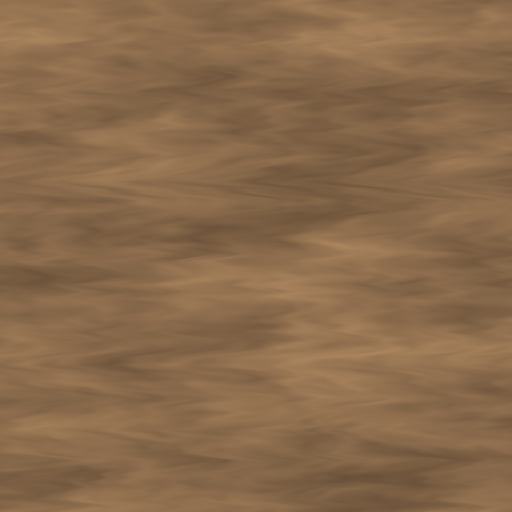
\includegraphics[width=0.35\textwidth]{figures/appendix/wood-param-control/wood-texture_base.png}
    \caption{Wood texture base configuration used as reference for the parameter comparisons.}
    \label{fig:wood-base}
\end{figure}

\begin{figure}[htbp]
    \centering
    \begin{tabular}{cc}
        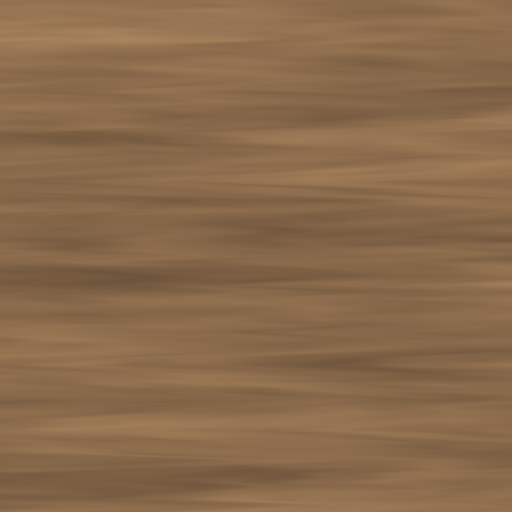
\includegraphics[width=0.45\textwidth]{figures/appendix/wood-param-control/wood-texture_anisotropy_0.10.png} &
        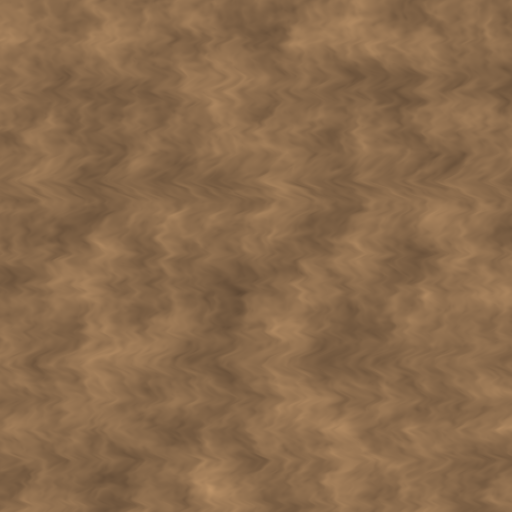
\includegraphics[width=0.45\textwidth]{figures/appendix/wood-param-control/wood-texture_anisotropy_1.00.png} \\[0.5em]
        Low value: 0.10 & High value: 1.00
    \end{tabular}
    \caption{Wood texture comparison for the anisotropy parameter. Lower values produce more directional stretching, while higher values reduce this directional compression.}
    \label{fig:wood-anisotropy}
\end{figure}

\begin{figure}[htbp]
    \centering
    \begin{tabular}{cc}
        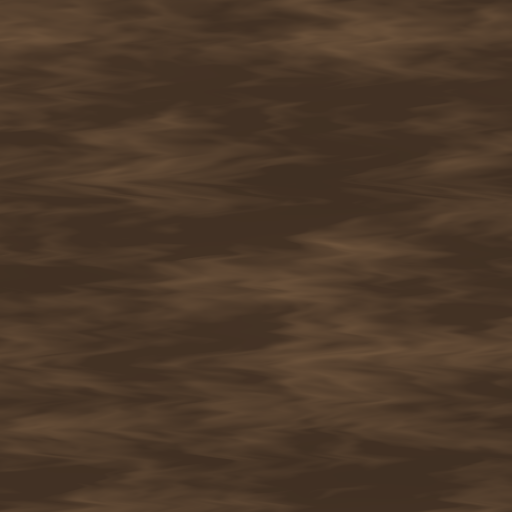
\includegraphics[width=0.45\textwidth]{figures/appendix/wood-param-control/wood-texture_brightness_-0.50.png} &
        
\includegraphics[width=0.45\textwidth]{figures/appendix/wood-param-control/wood-texture_brightness_0.50.png} \\[0.5em]
        Low value: -0.50 & High value: 0.50
    \end{tabular}
    \caption{Wood texture comparison for the brightness parameter. Lower values darken the generated texture, while higher values brighten the overall result.}
    \label{fig:wood-brightness}
\end{figure}

\begin{figure}[htbp]
    \centering
    \begin{tabular}{cc}
        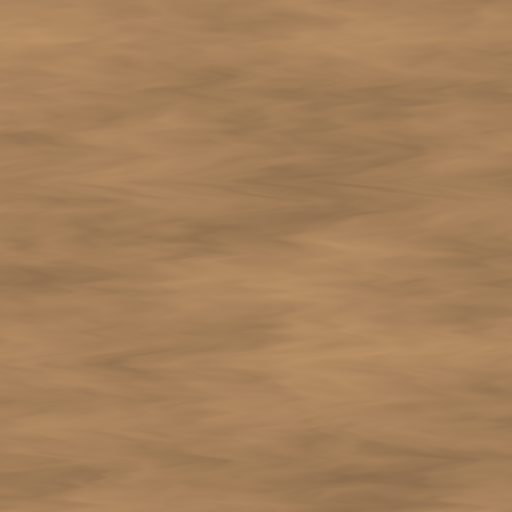
\includegraphics[width=0.45\textwidth]{figures/appendix/wood-param-control/wood-texture_contrast_0.50.png} &
        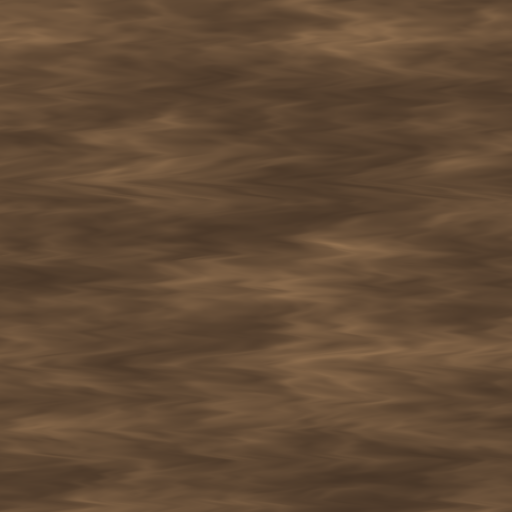
\includegraphics[width=0.45\textwidth]{figures/appendix/wood-param-control/wood-texture_contrast_3.00.png} \\[0.5em]
        Low value: 0.50 & High value: 3.00
    \end{tabular}
    \caption{Wood texture comparison for the contrast parameter. Lower values soften the difference between light and dark regions, while higher values make the grain pattern more pronounced.}
    \label{fig:wood-contrast}
\end{figure}

\begin{figure}[htbp]
    \centering
    \begin{tabular}{cc}
        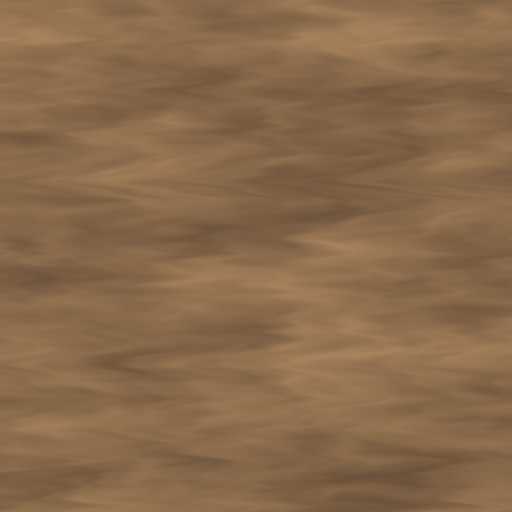
\includegraphics[width=0.45\textwidth]{figures/appendix/wood-param-control/wood-texture_crack_scale_2.00.png} &
        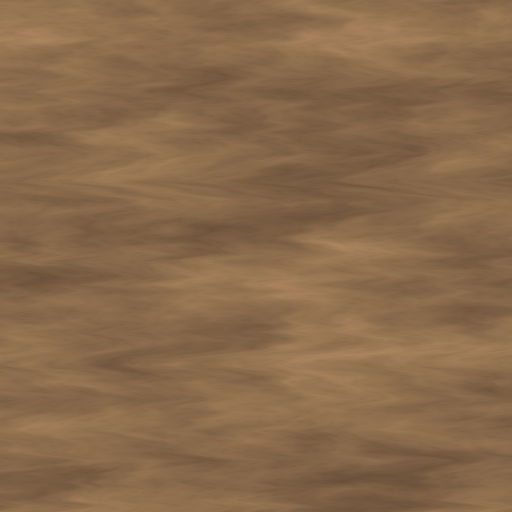
\includegraphics[width=0.45\textwidth]{figures/appendix/wood-param-control/wood-texture_crack_scale_15.00.png} \\[0.5em]
        Low value: 2.00 & High value: 15.00
    \end{tabular}
    \caption{Wood texture comparison for the crack scale parameter. Lower values create larger crack structures, while higher values create smaller and more frequent crack details.}
    \label{fig:wood-crack-scale}
\end{figure}

\begin{figure}[htbp]
    \centering
    \begin{tabular}{cc}
        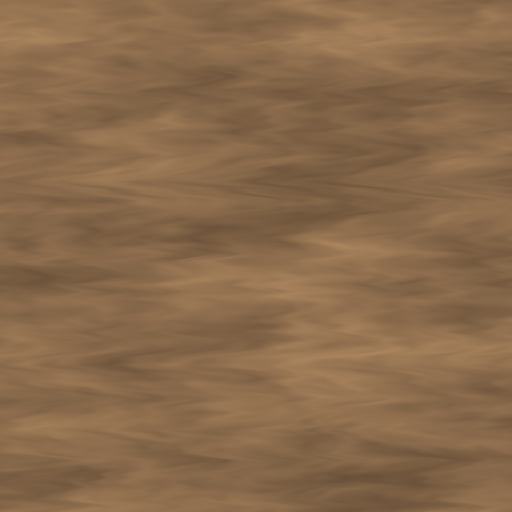
\includegraphics[width=0.45\textwidth]{figures/appendix/wood-param-control/wood-texture_crack_strength_0.00.png} &
        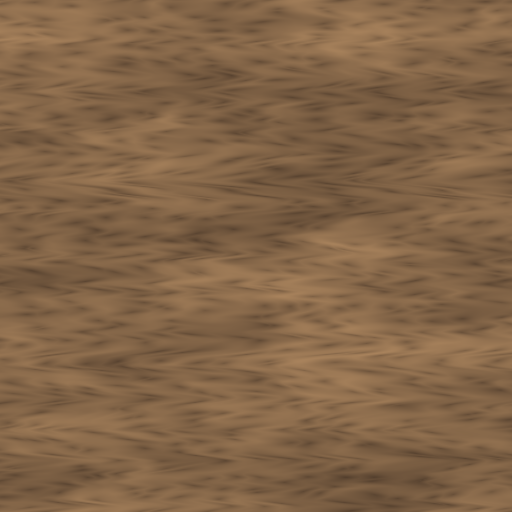
\includegraphics[width=0.45\textwidth]{figures/appendix/wood-param-control/wood-texture_crack_strength_0.50.png} \\[0.5em]
        Low value: 0.00 & High value: 0.50
    \end{tabular}
    \caption{Wood texture comparison for the crack strength parameter. Lower values remove crack influence, while higher values make crack-like structures more visible.}
    \label{fig:wood-crack-strength}
\end{figure}

\begin{figure}[htbp]
    \centering
    \begin{tabular}{cc}
        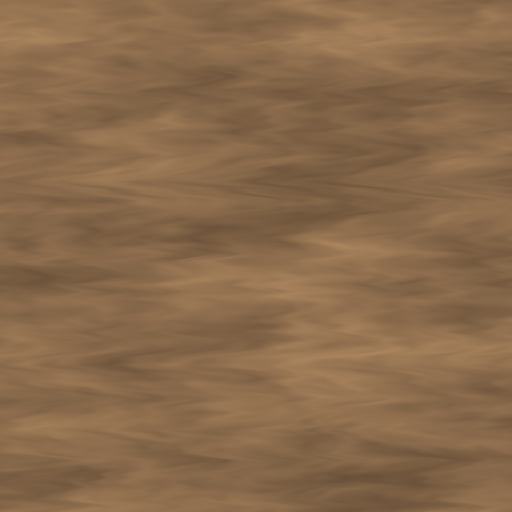
\includegraphics[width=0.45\textwidth]{figures/appendix/wood-param-control/wood-texture_detail_strength_0.00.png} &
        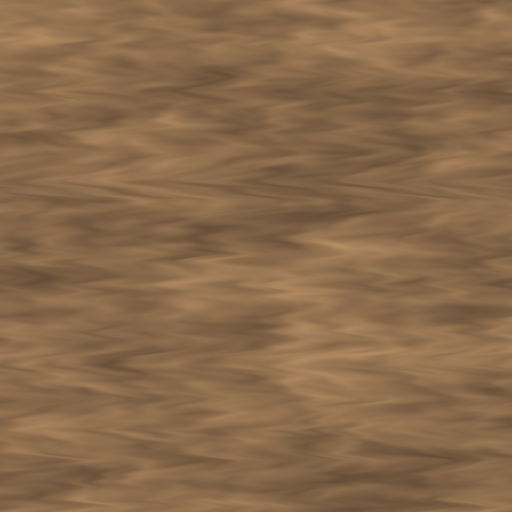
\includegraphics[width=0.45\textwidth]{figures/appendix/wood-param-control/wood-texture_detail_strength_0.50.png} \\[0.5em]
        Low value: 0.00 & High value: 0.50
    \end{tabular}
    \caption{Wood texture comparison for the detail strength parameter. Lower values reduce fine surface detail, while higher values add more small-scale variation to the grain.}
    \label{fig:wood-detail-strength}
\end{figure}

\begin{figure}[htbp]
    \centering
    \begin{tabular}{cc}
        
\includegraphics[width=0.45\textwidth]{figures/appendix/wood-param-control/wood-texture_grain_1.00.png} &
        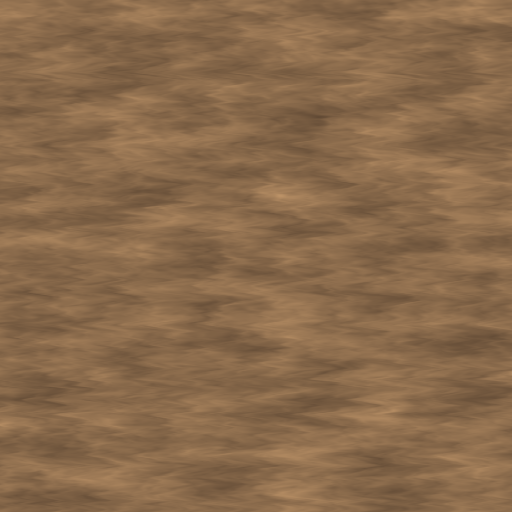
\includegraphics[width=0.45\textwidth]{figures/appendix/wood-param-control/wood-texture_grain_20.00.png} \\[0.5em]
        Low value: 1.00 & High value: 20.00
    \end{tabular}
    \caption{Wood texture comparison for the grain scale parameter. Lower values produce larger grain structures, while higher values produce finer and more frequent grain lines.}
    \label{fig:wood-grain}
\end{figure}

\begin{figure}[htbp]
    \centering
    \begin{tabular}{cc}
        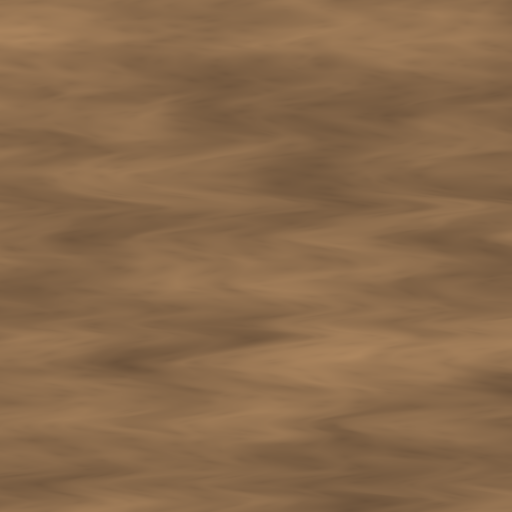
\includegraphics[width=0.45\textwidth]{figures/appendix/wood-param-control/wood-texture_Lacunarity_1.50.png} &
        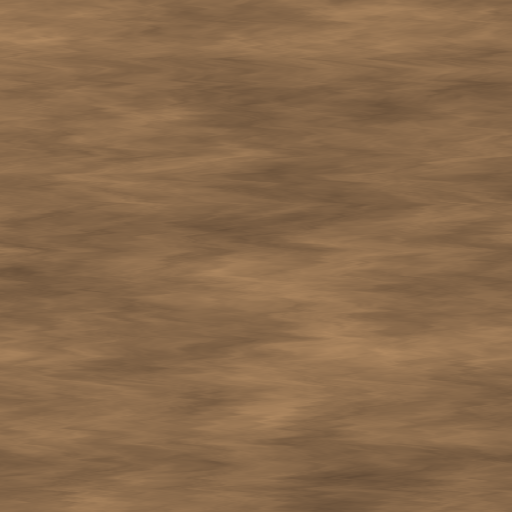
\includegraphics[width=0.45\textwidth]{figures/appendix/wood-param-control/wood-texture_Lacunarity_3.00.png} \\[0.5em]
        Low value: 1.50 & High value: 3.00
    \end{tabular}
    \caption{Wood texture comparison for the lacunarity parameter. Lower values keep octave frequencies closer together, while higher values increase frequency separation and create sharper multi-scale detail.}
    \label{fig:wood-lacunarity}
\end{figure}

\begin{figure}[htbp]
    \centering
    \begin{tabular}{cc}
        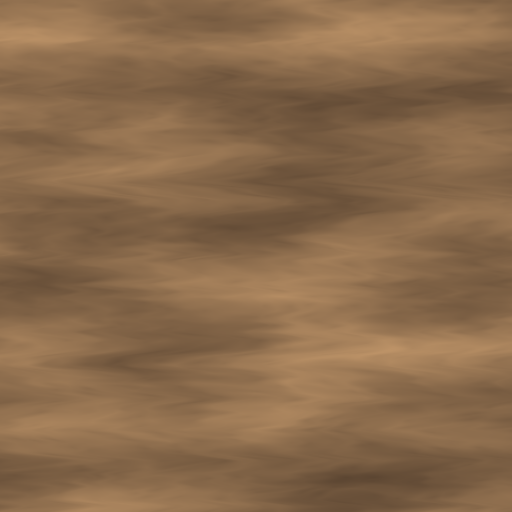
\includegraphics[width=0.45\textwidth]{figures/appendix/wood-param-control/wood-texture_octaves_1.png} &
        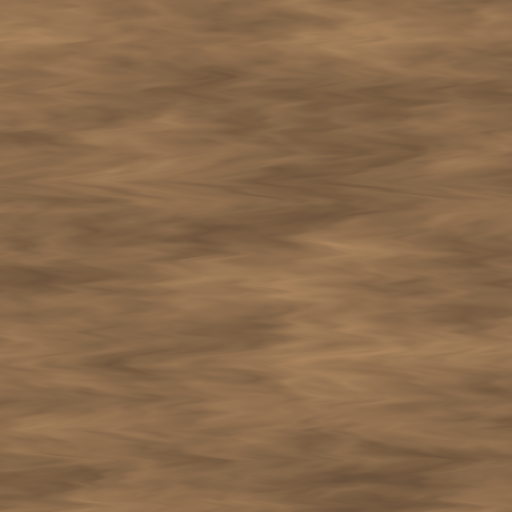
\includegraphics[width=0.45\textwidth]{figures/appendix/wood-param-control/wood-texture_octaves_6.png} \\[0.5em]
        Low value: 1 & High value: 6
    \end{tabular}
    \caption{Wood texture comparison for the octaves parameter. Lower values use fewer noise layers, while higher values add more layered detail to the texture.}
    \label{fig:wood-octaves}
\end{figure}

\begin{figure}[htbp]
    \centering
    \begin{tabular}{cc}
        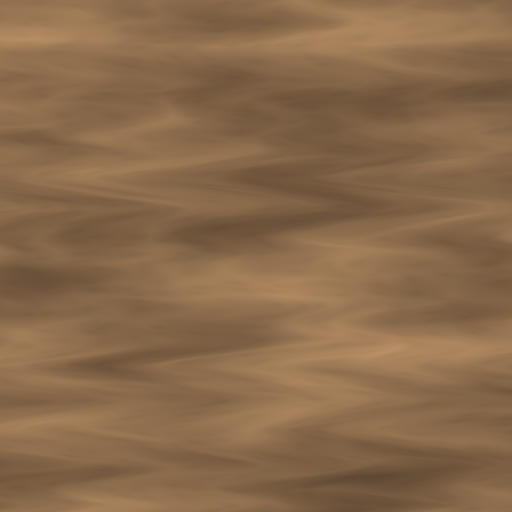
\includegraphics[width=0.45\textwidth]{figures/appendix/wood-param-control/wood-texture_persistence_0.10.png} &
        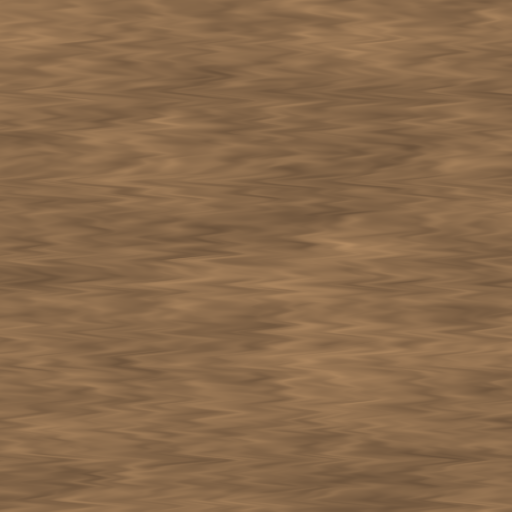
\includegraphics[width=0.45\textwidth]{figures/appendix/wood-param-control/wood-texture_persistence_0.90.png} \\[0.5em]
        Low value: 0.10 & High value: 0.90
    \end{tabular}
    \caption{Wood texture comparison for the persistence parameter. Lower values reduce the influence of higher-frequency layers, while higher values make fine details stronger.}
    \label{fig:wood-persistence}
\end{figure}

\begin{figure}[htbp]
    \centering
    \begin{tabular}{cc}
        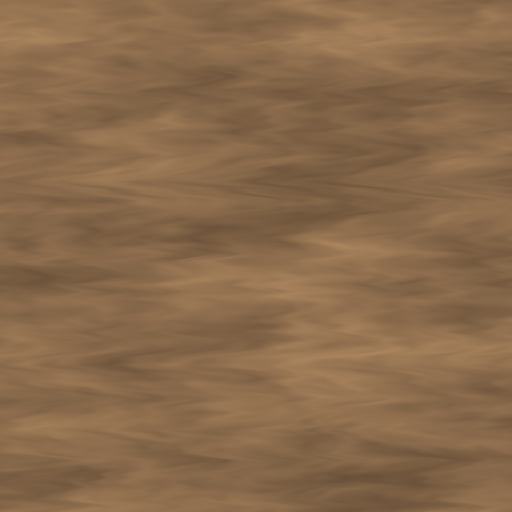
\includegraphics[width=0.45\textwidth]{figures/appendix/wood-param-control/wood-texture_ridge_strength_0.00.png} &
        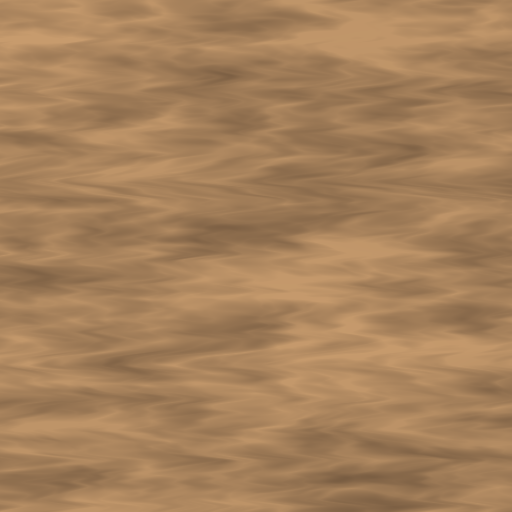
\includegraphics[width=0.45\textwidth]{figures/appendix/wood-param-control/wood-texture_ridge_strength_1.00.png} \\[0.5em]
        Low value: 0.00 & High value: 1.00
    \end{tabular}
    \caption{Wood texture comparison for the ridge strength parameter. Lower values reduce darker groove structures, while higher values emphasize ridges and grain boundaries.}
    \label{fig:wood-ridge-strength}
\end{figure}

\begin{figure}[htbp]
    \centering
    \begin{tabular}{cc}
        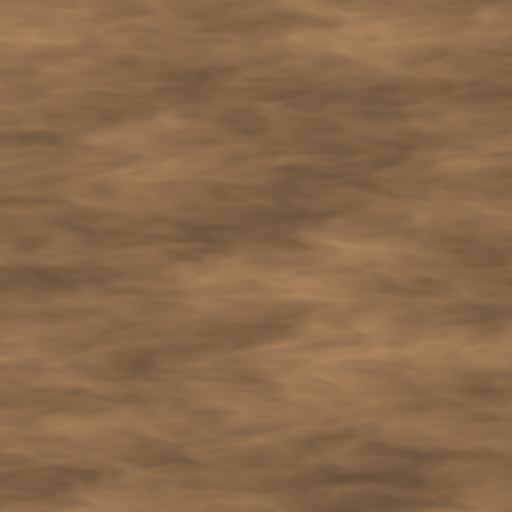
\includegraphics[width=0.45\textwidth]{figures/appendix/wood-param-control/wood-texture_warp_scale_0.50.png} &
        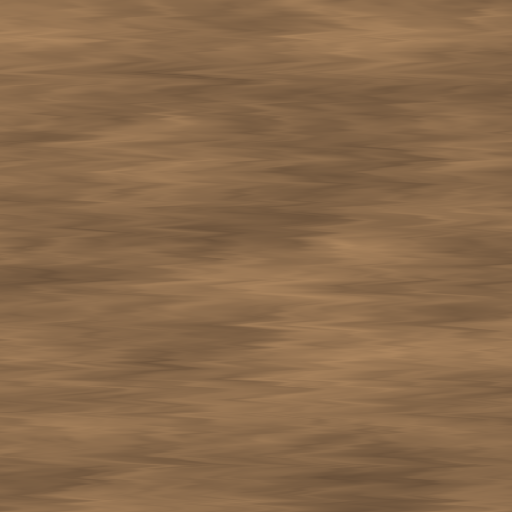
\includegraphics[width=0.45\textwidth]{figures/appendix/wood-param-control/wood-texture_warp_scale_5.00.png} \\[0.5em]
        Low value: 0.50 & High value: 5.00
    \end{tabular}
    \caption{Wood texture comparison for the warp scale parameter. Lower values create broad distortion waves, while higher values create more frequent local warping.}
    \label{fig:wood-warp-scale}
\end{figure}

\begin{figure}[htbp]
    \centering
    \begin{tabular}{cc}
        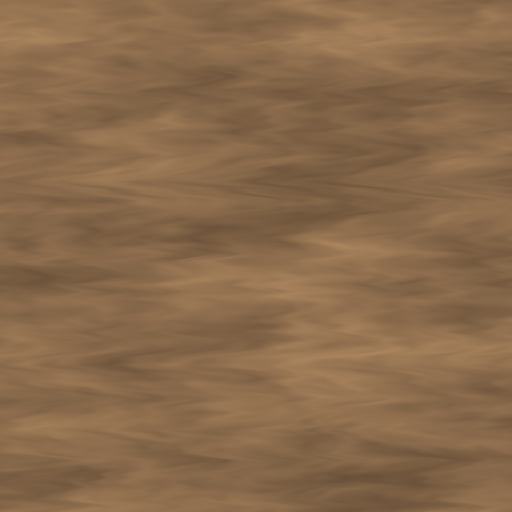
\includegraphics[width=0.45\textwidth]{figures/appendix/wood-param-control/wood-texture_warp_strength_0.00.png} &
        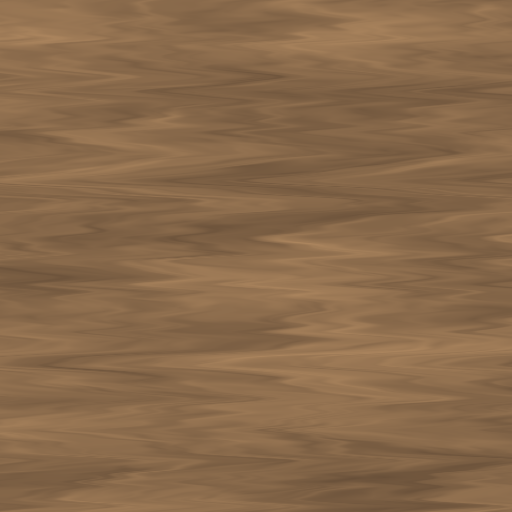
\includegraphics[width=0.45\textwidth]{figures/appendix/wood-param-control/wood-texture_warp_strength_2.00.png} \\[0.5em]
        Low value: 0.00 & High value: 2.00
    \end{tabular}
    \caption{Wood texture comparison for the warp strength parameter. Lower values keep the grain mostly regular, while higher values create stronger organic distortion.}
    \label{fig:wood-warp-strength}
\end{figure}

\clearpage
\section{Appendix C - GitHub Repository, Raw Data}
\subsection{Repository Structure for Evaluation Data}
\label{appendix:repository-structure}

The evaluation data and scripts used for the thesis are stored in the project repository. The most relevant folders are listed below to make the experimental data easier to locate and reproduce.

\begin{table}[H]
\centering
\caption{Repository structure for evaluation data and generated thesis artifacts}
\label{tab:repository_structure}
\begin{tabularx}{\textwidth}{|X|X|}
\hline
\textbf{Path} & \textbf{Content} \\
\hline
\hline
\texttt{evaluation/results/desktop/} & Raw CSV measurement data from the desktop evaluation runs. \\
\hline
\texttt{evaluation/results/desktop/checkpoint-*} & Individual checkpoint folders containing repeated run files and configuration files for each experiment. \\
\hline
\texttt{evaluation/results/desktop/evaluation-output/} & Aggregated CSV files and generated plots used in Chapter~6. \\
\hline
\texttt{docs/figures/06/} & Final evaluation figures included in the thesis. \\
\hline
\texttt{docs/figures/appendix/} & Additional appendix figures, including Wood parameter examples and optimization results. \\
\hline
\texttt{docs/tex/chapters/} & LaTeX source files for the written thesis chapters. \\
\hline
\end{tabularx}
\end{table}

\clearpage
\section{Appendix D - Project Management}
\subsection{Planning}

The project was planned in several phases, starting with ideation and research, followed by implementation, evaluation, and final handoff. Figure~\ref{fig:project-planning-phases} shows the high-level project timeline.

\begin{figure}[H]
    \centering
    \img[width=1\textwidth]{figures/appendix/timeplan-phases.png}
    {High-level project planning phases from ideation to final handoff.}
    \label{fig:project-planning-phases}
\end{figure}

\clearpage
\subsection{Work-Journal}

The following weekly work log summarizes the main activities carried out during the project. It is intended as a compact overview of the project progress rather than a detailed daily journal.

\begin{table}[H]
\centering
\caption{Weekly work log}
\label{tab:weekly_work_log}
\begin{tabularx}{\textwidth}{|l|X|}
\hline
\textbf{Week} & \textbf{Main activities} \\
\hline
\hline
Week 1 & Finalized assignment understanding, clarified thesis topic, and prepared the first research pitch. \\
\hline
Week 2 & Started initial research on algorithmic texture synthesis methods and existing tools. \\
\hline
Week 3 & Refined research questions, defined the intended use case, and prepared the conceptual direction of the prototype. \\
\hline
Week 4 & Continued research on procedural, rule-based, and optimization-based texture synthesis approaches. Found example-based texture synthesis approach as additional possible method. \\
\hline
Week 5 & Investigated existing tools and frameworks and identified limitations for controlled evaluation. \\
\hline
Week 6 & Started prototype implementation and basic architecture setup. \\
\hline
Week 7 & Implemented initial procedural environment and basic rendering setup. \\
\hline
Week 8 & Implemented first procedural texture generation methods and parameter controls. \\
\hline
Week 9 & Extended texture synthesis methods and connected generated textures to the terrain explorer. \\
\hline
Week 10 & Improved runtime measurement, texture generation workflow, and reproducibility handling. \\
\hline
Week 11 & Implemented and refined texture reuse, caching behaviour, and evaluation data export. \\
\hline
Week 12 & Added optimization-based approximation experiments and prepared evaluation configurations. \\
\hline
Week 13 & Finished main implementation work and started structured evaluation runs. \\
\hline
Week 14 & Started running tests to collect evaluation results, started writing the evaluation sections. \\
\hline
Week 15 & Finalized evaluation and test runs. Finalized thesis text, appendix material, figures, references, and final deliverables (Web-Abstract, PITCH-Video). \\
\hline
\end{tabularx}
\end{table}

\clearpage
\section{Appendix E - Official Assignment}
The original assignment document is included here for reference. The original (German, see next page):

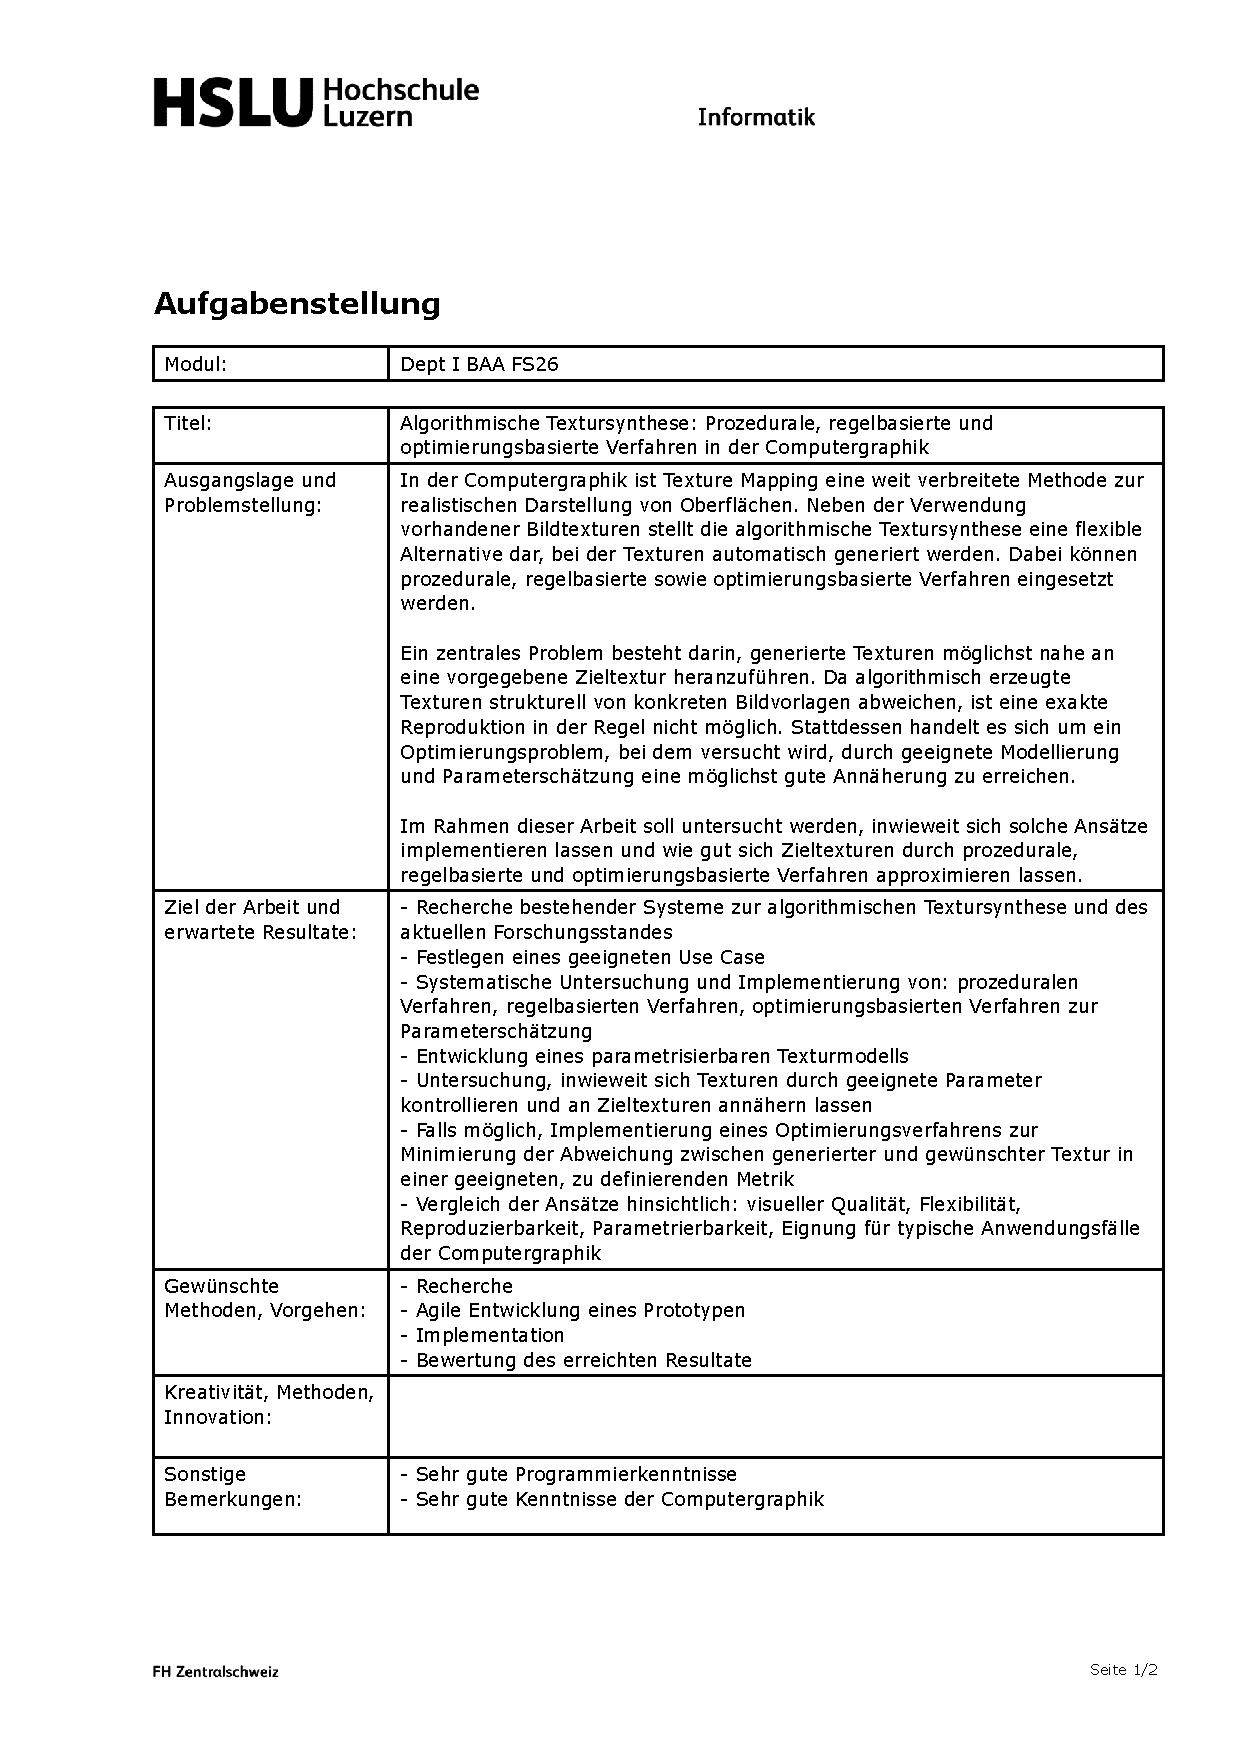
\includepdf[
  pages=-,
  scale=0.85,
  pagecommand={\thispagestyle{plain}}
]{tex/chapters/anhaenge/assignments/Aufgabenstellung_BAA_ORIGINAL.pdf}

\clearpage
Translated version (English, see next page):

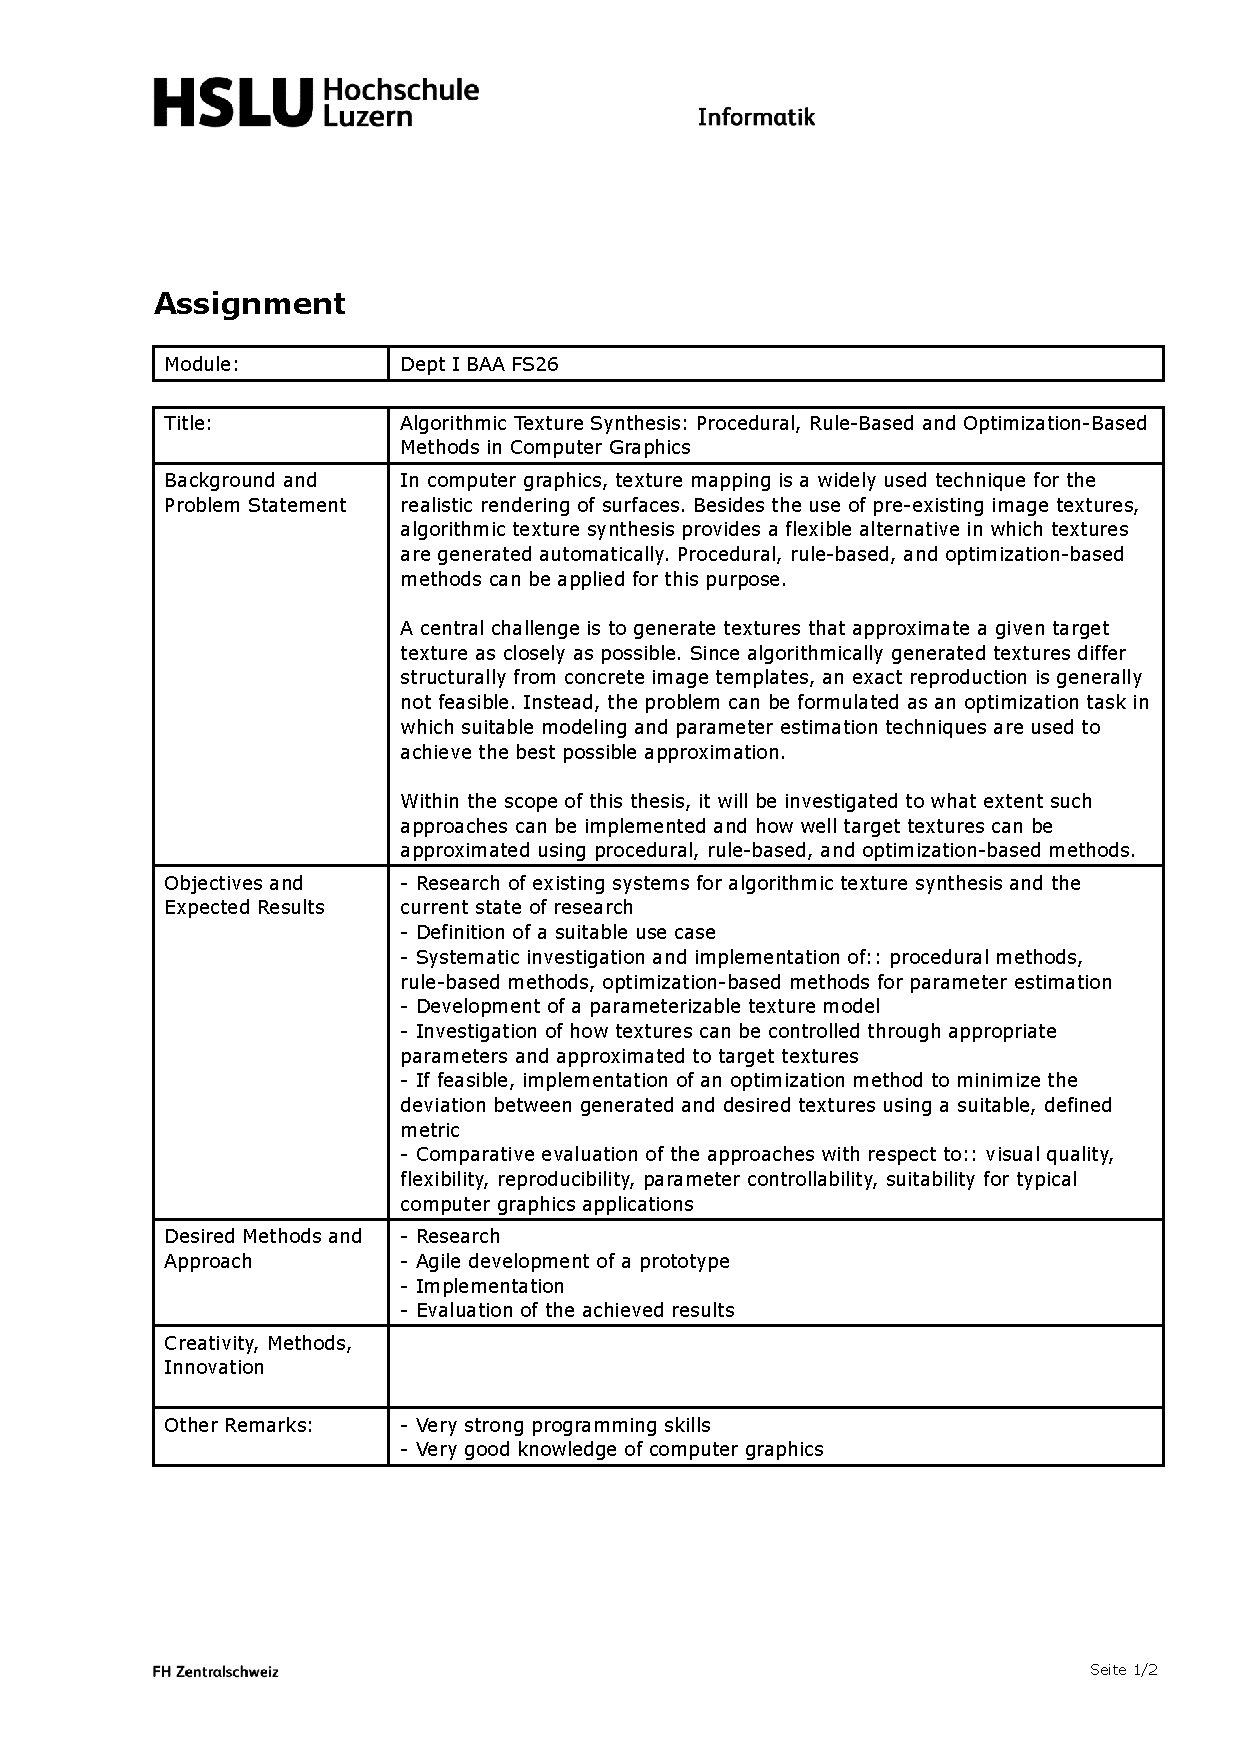
\includepdf[
  pages=-,
  scale=0.85,
  pagecommand={\thispagestyle{plain}}
]{tex/chapters/anhaenge/assignments/Aufgabenstellung_BAA_ENGLISH.pdf}


\chapter{References}
\raggedright
\section{List of Sources}

\printbibliography[heading=none]

\clearpage
\section{List of Figures}
\onlylof


\section{List of Tables}
\onlylot


\section{List of Code-Blocks}
\onlylol

\section{List of Acronyms}
\begingroup
% This tells the glossary to print absolutely no title and not trigger a chapter break
\renewcommand{\glossarysection}[2][]{}
\printglossary[type=\acronymtype]
\endgroup

\end{document}
